\documentclass[12pt,letterpaper,oneside]{report}
\usepackage[T1]{fontenc}
\usepackage[utf8]{inputenc}
%\DeclareUnicodeCharacter{0301}{\'{e}}
\usepackage[spanish,es-tabla]{babel}
\usepackage{caption} %% Descripcion de figuras
\usepackage{helvet} %% Letra Arial
\renewcommand{\familydefault}{\sfdefault} %%Letra Arial
\usepackage{graphicx} %% Figuras
\usepackage{float} %% Figuras
\usepackage{siunitx} %% Simbolo de Grado
\usepackage[left=2.54cm,right=2.54cm,top=2.54cm,bottom=2.54cm]{geometry} %% Margenes
\linespread{1.5} %% Interlineado
%\renewcommand{\baselinestretch}{1.5}
\usepackage{multirow}% Para las tablas
\usepackage{array}%alinear tablas
\usepackage{booktabs}% Para las tablas
\usepackage{tabularx}% Para las tablas
\usepackage{ragged2e}% Para las tablas
\usepackage{multicol}% Para las tablas
\usepackage{lineno} % Para las tablas
\usepackage{amsmath} % Para ecuaciones
\usepackage{amsfonts} % Para ecuaciones
\usepackage{amssymb} % Para ecuaciones
\usepackage[style=apa, backend=biber]{biblatex} %% bibliografia con biblatex%% %%% Opciones>Configurar>Biblatex> -biber %- -----%%
\DeclareLanguageMapping{spanish}{spanish-apa} %% bibliografia con biblatex%%
\usepackage{url} % para que salga bien la url y el doi%%
\urlstyle{same} % para que salga bien la url y el doi%%
\usepackage{csquotes} % Para la bibliografia
\addbibresource{Libreria_1.bib}
\usepackage{longtable} %% tablas largas
\parindent=0mm %% Sangria
\setcounter{tocdepth}{3} %% para que aparesca mas subindices
\setcounter{secnumdepth}{3}  %%para que aparesca mas subnideces
\usepackage{blindtext}
\usepackage{appendix}
\usepackage{pdflscape}
\usepackage[version=4]{mhchem}
\usepackage{fancyhdr}
\fancyhf{}
\fancyhead[R]{\leftmark}
\fancyhead[R]{\nouppercase{\rightmark}}
\fancyfoot[C]{\thepage}
\pagestyle{fancy}
\setlength{\headheight}{15pt}
\usepackage{titlesec}
\titleformat{\chapter}[block]
  {\normalfont\huge\bfseries}{\thechapter.}{1em}{\Huge}
\titlespacing*{\chapter}{0pt}{0pt}{30pt}
\begin{document}
\begin{titlepage}
\begin{center}
\vspace*{-2.5cm}
\begin{figure}[htb]
\begin{center}

\includegraphics[width=6.5cm]{figuras/UPP}
\end{center}
\end{figure}
\begin{Large}
Memoria de Estadía\\
\vspace*{0.25cm}
\textbf{Determinación de las funciones metabólicas de comunidades bacterianas asociadas a una milpa tradicional ubicada en El Boxo, Hidalgo} \\
\vspace*{0.25cm}
Presentada por:\\
\vspace*{0.25cm}
Eduardo Gustavo Bautista Barrera\\
\vspace*{0.25cm}
Para obtener el título de:\\
\vspace*{0.25cm}
Ingeniero en Biotecnología\\
\vspace*{0.25cm}
Asesores:\\
\vspace*{0.5cm}
Dr. Eneas Aguirre von Wobeser\\
Dr. Miguel Ángel Anducho Reyes
\vfill
\footnotesize{Zempoala, Hidalgo. \hfill Diciembre 2019}
\end{Large}
\end{center}
\end{titlepage}
\thispagestyle{empty} % para quitar numero a la pagina
\title{Determinación de las funciones metabólicas de \\ comunidades bacterianas asociadas a una \\ milpa tradicional ubicada en El Boxo, Hidalgo}
\author{Eduardo G. Bautista Barrera}
\date{}
\maketitle
\thispagestyle{empty}
\pagenumbering{Roman}
\chapter*{}
\begin{center}
\emph{\LARGE A mi familia}\\[1cm]
\end{center}
\begin{flushright}
Que me han apoyado a lo largo de mi vida
\end{flushright}
\chapter*{Agradecimientos} 
A la Universidad Politécnica de Pachuca, que me abrió sus puertas.
\\[1cm]
Al Dr. Eneas Aguirre von Wobeser, por su apoyo y por ser mi asesor y ayudarme en este trabajo.
\\[1cm]
Al Dr. Miguel Angel Anducho Reyes por su consejo y ayuda en la elaboración de esta memoria.
\\[1cm]
Al laboratorio AIRB por facilitar sus instalaciones.
\\[1cm]
A los colaboradores del CIDEA por el apoyo en la secuenciación.
\\[1cm]
A mis padres y mi hermana por confiar en mí y siempre apoyarme durante todos estos años de vida.
\\[1cm]
A mis abuelitos y a mis tíos por su ayuda y consejos.
\\[1cm]
A mis amigos de la carrera Karla Veloz Badillo, Daniel Jean-Baptiste, Victor Hidalgo Vera por su amistad y en especial a Karen Hernández Téllez por su apoyo incondicional y amor.
\chapter*{Resumen}
\addcontentsline{toc}{chapter}{Resumen} 
Este proyecto se enfoca en la predicción de las funciones metabólicas que realizan las comunidades bacterianas que están asociadas al suelo de una milpa localizada en la comunidad de El Boxo del municipio de Cardonal Estado de Hidalgo, para lo cual se tomaron muestras de suelo en asociación con las raíces de maíz, y a una distancia de 30 cm de cada planta como controles. Se extrajo ADN metagenómico, del cual se amplificó la región V4 del gen 16S ribosomal, y se secuenció en Illumina MiSeq. Los datos obtenidos se introdujeron en la plataforma bioinformática QIIME 2, y se utilizó PICRUSt para predecir las rutas metabólicas que desempeñan las comunidades bacterianas. Se encontró que las bacterias que crecen en la vecindad de plantas de maíz tienden a poseer más genes relacionados con el metabolismo de compuestos orgánicos, esto sugiere que dichos organismos consumen compuestos derivados de las plantas. Asimismo, se encontraron genes cerca de las raíces posiblemente involucrados en la interacción planta-microorganismo. Los resultados contribuyen al conocimiento de las comunidades rizosféricas asociadas a la raíz de maíz cultivada en la milpa, un agroecosistema particular en donde interactúan más de un cultivo.
\\[2cm]
\textbf{Palabras clave:} Milpa, Rutas metabólicas, Metagenómica, Ecologia microbiana, Agrobiotecnología.
\chapter*{Abstract}
\addcontentsline{toc}{chapter}{Abstract}
This project focuses on the prediction of metabolic functions performed by bacterial communities that are associated with the soil of a milpa located in the community of El Boxo in the municipality of Cardonal state of Hidalgo, for which soil samples were taken in association with corn roots, and at a distance of 30 cm from each plant as controls. Metagenomic DNA was extracted, from which region V4 of the 16S ribosomal gene was amplified, and sequenced in Illumina MiSeq. The data obtained were entered into the QIIME 2 bioinformatics platform, and PICRUSt was used to predict the metabolic pathways of bacterial communities. It was found that bacteria growing in the neighborhood of corn plants tend to have more genes related to the metabolism of organic compounds, suggesting that such organisms consume compounds derived from plants. Genes were also found near the roots possibly involved in the plant-microorganism interaction. The results contribute to the knowledge of the rhizospheric communities associated with corn root grown in the milpa, a particular agroecosystem in which more than one crop interacts.
\\[2cm]
\textbf{Keywords:} Milpa, Metabolic pathways, Metagenomics, Microbial ecology, Agrobiotechnology.
\renewcommand{\contentsname}{Contenido}
\tableofcontents
\cleardoublepage
\listoffigures
\addcontentsline{toc}{chapter}{Índice de figuras}
\cleardoublepage
\listoftables
\addcontentsline{toc}{chapter}{Índice de tablas}
\chapter*{Introducción}
\addcontentsline{toc}{chapter}{Introducción}
\markboth{Introducción}{Introducción}
\pagenumbering{arabic}
El crecimiento demográfico que México ha experimentado en los últimos años, aunado a las crisis económicas que enfrenta periódicamente, crea una demanda de alimentos difícil de satisfacer \autocite{Davis2016,Ibarrola-Rivas2017}. Para mantener la seguridad alimentaria, buscando conservar la independencia de las importaciones, es imperativo impulsar el campo agrícola \autocite{Gil-Mendez2015}. Con este fin, se plantean diferentes acciones, para obtener un mejor rendimiento en los cultivos y aumentar la superficie cultivada \autocite{Edgerton2009}. Desde los años ochenta, la producción de maíz en México se ha incrementado de 12 a más de 25 millones de toneladas por año \autocite{Sweeney2013}. En comparación, Estados Unidos y China producen actualmente 370 y 242 millones de toneladas de maíz por año \autocite{USDA2018}.
\par
El maíz (\textit{Zea mays L.}) es un cereal de vital importancia en la alimentación de las familias mexicanas y su consumo es bastante extendido en todo el territorio nacional \autocite{Morejon-Pereda2017}. Aunado a ello, juega un papel central en la cultura de los mexicanos desde la época prehispánica, donde la idiosincrasia de los pueblos se construía en torno a este grano. Hoy en día, es un elemento presente en la vida de las comunidades rurales, donde muchas festividades están relacionadas con su ciclo de cultivo; además se preparan múltiples platillos basados en él, y las tareas comunitarias frecuentemente involucran participar en su siembra \autocite{Barkin2002}.
\par 
A pesar de la importancia del maíz para los mexicanos, la gran demanda nacional de este grano no satisface la producción del país, teniéndose que importar aproximadamente 14 millones de toneladas \autocite{SAGARPA2017}. Para incrementar la producción, en México el cultivo se ha tecnificado, principalmente mediante el desarrollo de infraestructura para riego y el uso de agroquímicos \autocite{Sweeney2013}. Otra estrategia que se ha implementado, es el desarrollo de híbridos con mayor productividad, e incluso la modificación genética, aunque esta última no está permitida para su siembra en México \autocite{Crow1998,Rani2017,Wang2017,Mastrodomenico2018}. 
\par
A causa de los monocultivos y los agroquímicos, el suelo agrícola va perdiendo su efectividad, por lo que las producciones se ven afectadas para un buen crecimiento de los cultivos de maíz \autocite{Sithole2017}. Tan solo en los últimos años se han utilizado alrededor de 90 mil toneladas de agroquímicos, lo que ha derivado en una contaminación del 45\% del territorio del país \autocite{Bocco2005,Ortiz2013}.
\par
Para incrementar la producción del maíz, también es posible utilizar estrategias menos dañinas para el medio ambiente. Por ejemplo, es posible rescatar líneas o variedades ancestrales, que pueden estar adaptadas al crecimiento en condiciones de estrés, como la falta de agua. Otra estrategia se basa en la utilización de microorganismos, que presentan actividades bioquímicas o fisiológicas que benefician a las plantas, y además pueden ser formulados como biofertilizantes \autocite{Babu2017a,Saraf2013}.
\par
Algunos ejemplos de actividades benéficas que las bacterias otorgan al suelo y a las plantas son: la fijación de nitrógeno \autocite{Martins2017,Pii2015}, la promoción de crecimiento de plantas \autocite{Breedt2017,Compant2005}, la solubilización de fosfato \autocite{Babu2017b} y el biocontrol de organismos patógenos \autocite{Douriet-Gamez2017,Li2016}.
\par
Para aprovecharlas de forma más efectiva en la agricultura, un primer paso es conocer las bacterias que conviven naturalmente con el maíz, y las funciones que realizan. Derivado de esto, se propone utilizar a la metagenómica, la cual es una herramienta de biología molecular de gran utilidad, ya que permite conocer la diversidad filogenética de un ambiente, con lo que se pueden realizar predicciones de las funciones metabólicas que estos microorganismos realizan \autocite{Langille2013}. De esta manera, podemos identificar los microorganismos que son propios del ambiente y que interactúan con las plantas. Esto permitirá diseñar estrategias para poder aislarlos y en el futuro elaborar biofertilizantes que recuperen los suelos erosionados y aumenten el rendimiento de los cultivos.
\par
En este proyecto, se estudió la función que desempeña la microbiota del suelo de una milpa, en la comunidad de El Boxo, en la región del Alto Mezquital, Estado de Hidalgo. Se seleccionó este lugar en especial, puesto que no ha sufrido perturbaciones en cuanto al uso de agroquímicos, y porque se conservan las técnicas de antaño para el sembrado y labrado de la milpa.
\chapter{Marco Teórico}
\section{Importancia de las milpas}
Una milpa se define como una parte de campo abierto donde se realizan policultivos, centrado en el maíz, el cual se siembra junto con otros vegetales \autocite{Nigh2013}.
\par
La milpa en México es un sistema de cultivo de gran importancia, puesto que, desde hace miles de años, ha representado un auge en cuanto a la domesticación de plantas, la agricultura y la economía se \autocite{Zizumbo-Villarreal2017}, además ofrece una dieta equilibrada a las personas que la manejan \autocite{Gutierrez-Serrano2009}.
\par
Su origen se remonta a la época donde el maíz y el frijol fueron domesticados y donde los antiguos pobladores dejaban de ser nómadas para empezar a asentarse en lugares específicos. A raíz de esto, se desarrollaron técnicas de cultivo que les traían beneficios tanto nutricionales como económicos. Desde entonces y hasta la actualidad, la milpa es un símbolo de tradición que representa a la cultura mexicana y a la agricultura en general \autocite{Escalante-Gonzalbo2008}.
\section{La milpa, sistema de policultivo}
El sistema agrícola milpa, se caracteriza principalmente porque convergen más de un solo cultivo, ya que por lo general se siembra la triada mesoamericana que incluye: frijol, calabaza y maíz; estas plantas tienen entre sí una relación sinérgica, puesto que el frijol ofrece nitrógeno al maíz el cual a su vez da soporte para la enredadera de esta leguminosa, de igual manera las hojas de la calabaza impiden que otras hierbas crezcan ofreciendo sombra al suelo, evitando así, la evaporación. Incluso, en algunas ocasiones se puede llegar a sembrar cempasúchil y otras hierbas para tener un control de plagas \autocite{Buenrostro2009}. Además, las milpas pueden contener decenas de otras especies, incluyendo: chile, cacahuate, lenteja, árboles frutales y distintos quelites, así como plantas medicinales \autocite{Teran1995}.
\section{El maíz}
El cultivo más importante de la milpa es el maíz, ya que este cereal es la base de la alimentación de muchos pueblos, incluyendo la mayor parte de los mexicanos. Es una planta originaria de Mesoamérica (Fig. 1), cuya domesticación se cree que comenzó hace aproximadamente nueve mil años \autocite{Matsuoka2002}. Se caracteriza por ser de tallos gruesos y llegar a medir 2.4 m de altura promedio. Es una planta que tiene inflorescencias, por lo tanto, posee ambos aparatos reproductores; la espiga en la cima es el macho, y la hembra que se encuentra en el tallo en forma de mazorca \autocite{Aguilar2003,Kato-Yamakake2009}.
\par
A partir de esta configuración biológica, el maíz se puede diversificar, llegando a crear variedades con características que se pueden adaptar a una gran variedad de regiones, con grandes diferencias en el clima, en las características fisicoquímicas del suelo, en las pendientes del terreno, etc. Además de las variedades nativas, que son generadas mediante selección natural durante generaciones, se han realizado programas de mejoramiento mediante cruzas, resultando en híbridos, que son de gran importancia para los agricultores \autocite{Schwember2011}.
\par
Por lo tanto, en México se cuenta con una gran variedad de razas criollas, además de las variedades híbridas desarrolladas agronómicamente. En ocasiones, las primeras suelen tener ventajas sobre las segundas, ya que éstas requieren una menor cantidad de agroquímicos y además se adaptan mejor a climas extremos. Algunas de las razas criollas que se cultivan son: Chalqueño, Tuxpeño, Comiteco, Conejo, Chapalote, Tabloncillo entre otros \autocite{Aguilar2003}.
\begin{figure}[!h]
\addcontentsline{lof}{section}{\textbf{Figura 1.-} Planta de maíz criollo.}
\centering
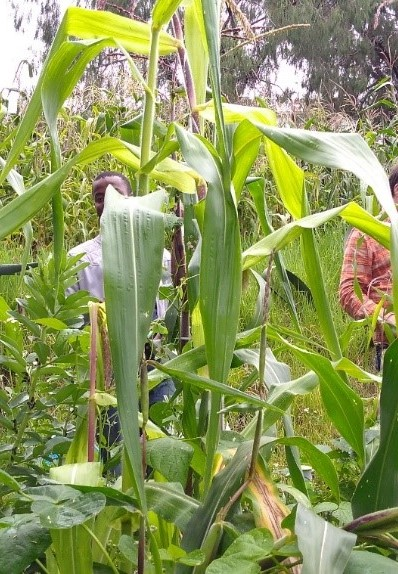
\includegraphics[width=5.6cm]{figuras/IMG_1}
\caption*{\textbf{Figura 1.-} Planta de maíz criollo (Fuente propia).}
\label{Figura 1}
\end{figure}
\newpage
\subsection{Producción de maíz en México}
Se estima que en México se cosechan entre 26.8 y 30 millones de toneladas de maíz al año. La producción de maíz se divide principalmente en grano amarillo y grano blanco (Tabla 1) \autocite{USDA2018}.
\par
\begin{table}[!h]
\addcontentsline{lot}{section}{\textbf{Tabla 1.-} Producción y superficie cultivada de maíz.}
\begin{center}
\caption*{\textbf{Tabla 1.-} Producción y superficie cultivada de maíz correspondiente al año 2017 en México \autocite{INEGI2018}.}
\label{Tabla 1}
\begin{tabular}{ccc}
\toprule[0.5mm]
Tipo de grano & Producción (toneladas) & Superficie (hectáreas)\\
\midrule
Amarillo & 8,071,840 & 1,502,236 \\
Blanco & 23,142,203 & 60,947,000 \\
\bottomrule[0.5mm]
\end{tabular}
\end{center}
\end{table}
La mayor parte de la producción de grano amarillo se destina al consumo pecuario y a la industria. Sin embargo, la demanda nacional solo es cubierta en un 24\% y por ello México importa alrededor de 13 millones de toneladas de grano, lo que lo convierte en el segundo importador de maíz más grande del mundo. El 98\% de las importaciones provienen de Estados Unidos, el resto de Argentina, Brasil y Canadá. El 52\% de la producción de grano blanco se destina principalmente a la venta para consumo humano, el cual satisface en su totalidad la demanda nacional. El resto es destinado al consumo pecuario, autoconsumo, exportación y siembra. Sin embargo, México importa de EE. UU. alrededor de 1 millón de toneladas de maíz blanco al año. Se estima que para 2030 la producción de grano blanco se duplique y que el consumo descienda, ocasionando que el excedente se exporte a países como Japón y Corea del Sur \autocite{SAGARPA2017}.
\subsection{Producción de maíz en el Estado de Hidalgo}
Hidalgo posee una extensión territorial de 2,098,700 ha, donde el 30\% representa el área destinada a la agricultura. El 20\% de la población hidalguense se encuentra laborando en el sector primario (Agricultura, ganadería y pesca). De este estrato, el 90\% se dedica a la agricultura, y de esta población, el 31.2\% produce maíz grano. En el 2018 la superficie cultivada de maíz en el año agrícola fue de 228,786 ha, de las cuales se obtuvo una producción de 630,835 toneladas, incluyendo maíz de riego y maíz de temporal (Tabla 2). Hidalgo ocupa el $\SI{12}{\degree}$ lugar nacional de producción de maíz grano, los municipios que presentan una mayor aportación, son: Tezontepec, Mixquiahuala, Tula y San Salvador \autocite{SIAP2017, INEGI2017}.
\begin{table}[h]
\addcontentsline{lot}{section}{\textbf{Tabla 2.-} Producción obtenida y la superficie utilizada en cultivo de riego y de temporal en Hidalgo.}
\begin{center}
\caption*{\textbf{Tabla 2.-} Producción obtenida y la superficie utilizada en cultivo de riego y de temporal en Hidalgo \autocite{INEGI2017}.}
\label{Tabla 2}
\begin{tabular}{ccc}
\toprule[0.5mm]
Sistema & Producción (t) & Superficie (ha)\\
\midrule
Riego & 430,659 & 59,613 \\
Temporal & 200,176 & 169,173 \\
\bottomrule[0.5mm]
\end{tabular}
\end{center}
\end{table}
\newpage
\subsection{El maíz, como monocultivo}
El maíz es comúnmente producido en monocultivo, que es aquel en donde se cultiva una sola especie de planta a la vez \autocite{Connor2011}. Sin embargo, este tipo de cultivo tiende a limitar los nutrientes del suelo, además de que son más propensos a la contaminación por plagas. Si bien se han desarrollado diversas tecnologías como la rotación de cultivo y el uso de agroquímicos, esto no exime al suelo de ser severamente dañado por el uso excesivo de éstos. Puesto que el objetivo de las grandes corporaciones es producir cantidades exorbitantes de producto en un intervalo de tiempo muy corto, esto inevitablemente hace que los suelos se desgasten, provocando así la disminución de la microbiota existente \autocite{Wang2014,Yang2016a,Zhang2017}.
\par  
\section{El suelo}
La salud de un agroecosistema depende en gran medida del manejo adecuado del suelo. Aunque el cultivo del maíz se puede realizar en una gran variedad de tipos de suelo, algunos suelos favorecen más la agricultura que otros. El suelo se define como una mezcla de diversos materiales orgánicos como: minerales, gases, líquidos y diversos organismos, que en conjunto sostienen la vida. Se caracteriza por ser un medio para el crecimiento de plantas y para el almacenamiento, suministro y purificación del agua \autocite{Tarbuck2005}. 
\par
Se compone principalmente de roca meteorizada, restos vegetales y animales; aunque su mayor componente es el aire y el agua.
La composición del suelo cambia a distintos niveles de profundidad y generalmente se le describe como distintas capas, llamadas horizontes. La capa más superficial del suelo se compone de materia orgánica; aquí se encuentran, por ejemplo: restos de hojas. La segunda se forma de minerales meteorizados, a partir de rocas más grandes. Después, continúa el subsuelo que es donde existe una mayor aglomeración de minerales y arcillas; en esta área es donde se llevan a cabo muchos de los procesos biológicos como la descomposición de la materia orgánica, así como los procesos metabólicos propios de los microorganismos que lo habitan. Posteriormente se encuentra el material no consolidado que proviene originalmente de la roca madre y debajo de este, se encuentra el lecho de roca \autocite{Smith2007}.
\par
La fracción de suelo más relevante para este proyecto es en la que se llevan a cabo los procesos biológicos en que participan tanto microorganismos como plantas.
\subsection{El suelo en la agricultura}
Las variables más importantes de un suelo destinado para la agricultura son: textura, profundidad, permeabilidad, actividad biológica, capacidad para retener agua y nutrientes, así como la cantidad de materia orgánica que contiene \autocite{NRC1993}. Los valores óptimos de estas variables que le dan al suelo características idóneas, y permiten tener sistemas de cultivo más productivos, así como también prevenir la erosión, se discuten a continuación. 
\subsubsection{Textura}
La textura del suelo viene dada de acuerdo con el tamaño de partículas que lo conforman. Dentro de esta clasificación de partícula se encuentran: arena muy gruesa, arena gruesa, arena mediana, arena fina, arena muy fina, limo y arcilla \autocite{Lindbo2012}. Las características texturales de estos tipos de suelo se pueden observar en la Tabla 3.
\par
Aunque la textura del suelo se puede determinar empíricamente (tocando el suelo), se deben realizar pruebas en laboratorio para una mayor precisión. Las texturas del suelo se clasifican en 3 grandes grupos: Arenoso, Franco y Arcilloso, y de acuerdo con las proporciones de cada uno de estos grupos, se subclasifican en: Arena, Franco arenoso, Franco, Franco limoso, Limoso, Franco arcilloso arenoso, Franco arcilloso, Franco arcilloso limoso, Arcilla arenosa, Limoso arcilloso y Arcilla. Todos estos grupos se representan en el triángulo de texturas (Fig. 2). Dependiendo de la textura del suelo, éste tendrá características distintas, por ejemplo, si el suelo presenta una mayor cantidad de arena, al ser más porosa, permite que el agua y los gases la atraviesen con mayor facilidad. Si presenta una mayor cantidad de limo, al poseer una porosidad reducida, provoca el aumento de agua y gases, lo que hace que sea mejor para el cultivo de plantas. Por último, la arcilla, cuyo tamaño de partícula es tan pequeño que no se puede observar a simple vista, favorece la compactación del aire, provocando que el agua se mueva con dificultad, lo que impide que las raíces logren absorber toda el agua contenida. Por ende, esta textura de suelo tiene un bajo rendimiento en cultivos \autocite{Chaudhari2013,Lindbo2012}.
\begin{table}[!h]
\addcontentsline{lot}{section}{\textbf{Tabla 3.-} Características de la textura del suelo.}
\centering
\small
\setlength\tabcolsep{3pt}
\setlength\extrarowheight{2pt}
\caption*{\textbf{Tabla 3.-} Características de la textura del suelo \autocite{Lindbo2012}.}\label{Tabla 3}
\begin{tabularx}{\linewidth}{*{5}{>{\hangindent=1em\hangafter=1\Centering}X}}
\toprule[0.5mm]
Partícula   & 
Diámetro (mm)    & 
Volumen (\si{\cubic\milli\metre})    &
Número de partículas por gramo   &
Área de superficie en 1 g (\si{\square\centi\metre})     \\ 
\midrule
Arena muy gruesa  & 2.00-1.00  & 4.18       & 90             & 11  \\
Arena gruesa      & 1.00-0.50  & 0.524      & 720            & 23   \\
Arena mediana     & 0.50-0.25  & 0.0655     & 5700           & 45    \\
Arena fina        & 0.25-0.10  & 0.00818    & 46,000         & 91     \\
Arena muy fina    & 0.10-0.05  & 0.000524   & 722,000        & 227     \\
Limo              & 0.05-0.002 & 0.000065   & 5,776,000      & 454      \\
Arcilla           & \textless0.002     & \num{4e-9} & 90,260,853,000 & 8,000,000 \\
\bottomrule[0.5mm]
\end{tabularx}
\end{table}

\begin{figure}[!h]
\addcontentsline{lof}{section}{\textbf{Figura 2.-} Tipo de textura de acuerdo a la composición de cada tipo de partícula del suelo.}
\centering
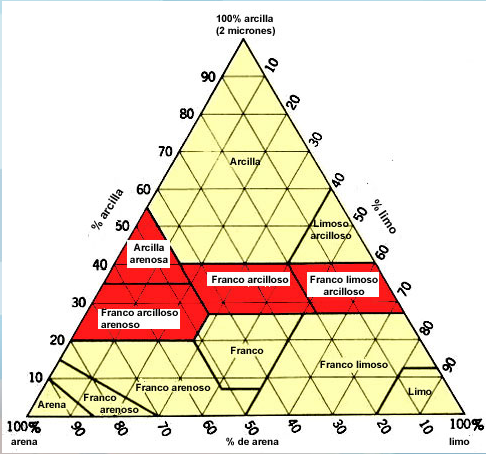
\includegraphics[width=9.42cm]{figuras/IMG_2}
\caption*{\textbf{Figura 2.-} Tipo de textura de acuerdo a la composición de cada tipo de partícula del suelo \autocite{FAO2006}.}
\label{Figura 2}
\end{figure}
\newpage
\subsubsection{Profundidad}
Para la profundidad del suelo, se consideran las capas en las que las raíces de las plantas penetran, para satisfacer sus necesidades biológicas. Básicamente está asociada con la capacidad de retención de agua. En algunos periodos del año, cuando las lluvias son más abundantes, el suelo absorbe y retiene el líquido. El ciclo de retención comienza cuando hay abundantes lluvias, en donde el agua se filtra y se deposita a cierta profundidad (Tabla 4). En su trayecto desde la superficie, se puede evaporar o ser absorbida por las raíces de las plantas. El agua que no es aprovechada llega hasta el subsuelo y recarga los manantiales que estén presentes en la zona \autocite{Lindbo2012,SSDS2017}.

\begin{table}[!h]
\addcontentsline{lot}{section}{\textbf{Tabla 4.-} Clasificación del suelo por su profundidad.}
\begin{center}
\caption*{\textbf{Tabla 4.-} Clasificación del suelo por su profundidad \autocite{Lindbo2012}.}
\label{Tabla 4}
\begin{tabular}{cc}
\toprule[0.5mm]
Clase & Profundidad (cm) \\
\midrule
Muy profundo & >150 \\
Profundo & 100-150  \\
Moderadamente profundo & 50-100  \\
Superficial & 25-50  \\
Muy superficial & 0-25 \\
\bottomrule[0.5mm]
\end{tabular}
\end{center}
\end{table}
\newpage
\subsubsection{Permeabilidad e infiltración}
La permeabilidad es la capacidad que posee un material para permitir el paso de un fluido a través de él lo cual depende de su porosidad. Por ejemplo, en suelos arenosos el agua atraviesa con rapidez debido a que sus poros son más grandes. En contraste, en suelos arcillosos el paso del agua es más lento por los poros, debido a que son más reducidos.
\par
A diferencia de la permeabilidad, la infiltración es el proceso en el que el agua de la superficie entra en el suelo. Esto depende de varios factores como la textura e incluso la materia orgánica que se encuentra en la superficie. Un alto grado de infiltración resiste a la erosión debido a que la velocidad de filtración del agua es más baja, de igual manera aumenta la cantidad que es irrigada al suelo \autocite{SSDS2017}.
\subsubsection{Materia orgánica}
La materia orgánica se forma principalmente, a partir de cualquier organismo que haya tenido vida y de los desechos que haya producido. La que está presente en el suelo es de vital importancia porque mejora la infiltración y previene de la erosión al fungir como protector. Algunas de las características benéficas que los contenidos elevados de materia orgánica proporcionan al suelo son las siguientes \autocite{Chaudhari2013,Lindbo2012}:
\begin{itemize}
\item Proporciona una fuente de carbono a los microorganismos del suelo
\item Mejora el paso del agua, ayudando así al crecimiento de las plantas
\item Almacena nutrientes que son esenciales, como el nitrógeno y el fósforo
\end{itemize}
\subsection{La rizosfera}
La rizosfera se define como aquella zona en el suelo donde coexisten las raíces y la biota que se encuentra a su alrededor. Aquí es donde se llevan a cabo todas las interacciones presentes entre ambos y en donde las plantas obtienen los nutrientes necesarios para vivir \autocite{Larsen2015,Lynch2012}.
\par
Se compone principalmente de hongos y bacterias, pero también están presentes arqueas, protozoos y virus, algunos de los cuales fungen como depredadores \autocite{Cardon2007}.
\par
Diversos estudios de poblaciones microbianas en la rizosfera se enfocan principalmente en el mejoramiento de la agricultura. Esto incluye el estudio de bacterias fijadoras de nitrógeno y carbono, bacterias que promueven el crecimiento de plantas y para biocontrol \autocite{Compant2005,Vejan2016}.
\newpage
\section{Comunidades bacterianas en suelos}
Las comunidades bacterianas asociadas al suelo juegan un papel de gran importancia, puesto que llevan a cabo diversas funciones, por ejemplo: intervienen en los ciclos biogeoquímicos, desarrollan los ecosistemas terrestres, contribuir a mantienen el suelo fértil, controlan la formación y la erosión del suelo, y además muchas especies son benéficas para la salud de las plantas \autocite{Buckley2003,Castaneda2017,Tecon2017}. Sin embargo, diversas actividades humanas como la agricultura afectan de manera considerable a las comunidades bacterianas, hacen que éstas reduzcan su actividad metabólica. Esto es ocasionado, entre otros factores, por fertilizantes que se agregan a los cultivos, causando una desestabilización en los ciclos del nitrógeno y del carbono \autocite{Alvarez-Yela2017}.
\par 
Una de las grandes ventajas de las comunidades bacterianas es que mantienen la salud de las plantas en buen estado. Esto es gracias a que estas ultimas poseen un mecanismo en el cual seleccionan el tipo de bacterias que estarán alrededor de sus raíces, provocando la formación de una red de defensa contra microorganismos patógenos. Este proceso de selección bacteriana no es del todo entendido, por lo que se debe profundizar su estudio. Esto permitirá identificar oportunidades para el desarrollo de productos biotecnológicos amigables con el medio ambiente, que permitan el mejoramiento del rendimiento de los cultivos \autocite{Berendsen2012,Berg2009}.
\par
Diversos microorganismos provenientes del suelo se han estudiado a fondo gracias a técnicas microbiológicas de cultivo. Sin embargo, muchas otras especies no se pueden cultivar debido en gran parte, a que las condiciones nutricionales en un medio de cultivo no son ideales para ellas, además de que en determinadas ocasiones necesitan estar en asociación con otras especies y por ende, no se reproducen en laboratorio \autocite{Stewart2012}. Por ello, es imperativo el uso de tecnologías revolucionarias que proporcionen información relevante sobre las bacterias que aún son desconocidas, así como saber qué tipo de interacciones ocurren en la rizosfera.
\section{Simbiosis, comunidades bacterianas - plantas}
Como se ha mencionado anteriormente, el suelo de las milpas se caracteriza por contener microbiota que contribuye al buen desarrollo de las plantas. Esto se debe a la interacción simbiótica que existe entre estos grupos de organismos, que entre otras ventajas permite a las plantas obtener nutrientes que son escasos, como el fósforo o el nitrógeno \autocite{Martin2017}.
\par
En este sentido, la simbiosis es una asociación entre especies distintas que conlleva el beneficio o no, de una o ambas partes. El tipo que ocurre entre muchas bacterias y las plantas es mutualista, es decir, que se lleva a cabo un vínculo entre integrantes de dos especies diferentes, en donde uno y otro son beneficiados \autocite{Smith2007}. Cabe resaltar que también existen bacterias patógenas para las plantas, las cuales a su vez pueden ser controladas por otras bacterias \autocite{Barka2015,Vejan2016}.
\par
Diversos estudios describen la importancia de las comunidades bacterianas en el suelo y la relación simbiótica que estas tienen con los cultivos. Por ejemplo, \textcite{Garbeva2007} mencionan que distintas especies de plantas exudan sustancias químicas, que atraen a una comunidad en específico para que ésta se adhiera a sus raíces y se lleve a cabo una simbiosis. Incluso se ha detectado que el maíz tiene la capacidad de seleccionar el tipo de bacterias que pueden estar a su alrededor \autocite{Aguirre-von-Wobeser2018,Niu2017}.
\newpage
\section{Funciones metabólicas de las comunidades bacterianas}
Las comunidades bacterianas realizan procesos que se traducen en funciones que ayudan al suelo a mantenerse fértil, y en un buen balance de nutrientes para sustentar la vida. Algunas de ellas son: comunicación, defensa y reproducción \autocite{Sanchez-de-Prager2012}. Sin embargo, el conocimiento del papel de las bacterias en el suelo es todavía limitado, y es posible que existan más funciones metabólicas que posean un potencial biotecnológico. Puesto que las raíces de las plantas segregan señales químicas que intervienen en las interacciones con las comunidades bacterianas, es importante investigar este tema en sistemas agrícolas \autocite{Petriacq2017}.
\par
Por otro lado, el metabolismo de las comunidades bacterianas se ve altamente afectado por las actividades agrícolas, en parte, debido al uso de fertilizantes ricos en nitrógeno, puesto que el uso excesivo hace que las bacterias fijadoras de \ce{N} se vean afectadas, propiciando la aparición de bacterias nitrificadoras que producen nitrato, y con este exceso de nitrato las bacterias denitrificadoras forman \ce{N2O}, el cual es un severo contaminante para los mantos acuíferos \autocite{DeGraaff2019,Vejan2016}.
\par
Por esto, es importante investigar la manera de cómo las bacterias interactuan con el suelo de manera benéfica para que contribuyan en el buen cultivo, en este caso del maíz.
\newpage
\section{Metagenómica}
La metagenómica, en esencia, permite la investigación del material genético de comunidades microbianas en conjunto, sin la necesidad de aislarlas en un cultivo. Debido al avance tecnológico que las nuevas técnicas de secuenciación presentan actualmente, es de mayor facilidad utilizar herramientas como ésta para determinar las secuencias de ADN ambiental. Con la metagenómica se obtiene información acerca de las bacterias que están presentes en el suelo, las funciones que realizan, así como también las interacciones que existen entre ellas \autocite{Hernandez-DeLira2014,Sharpton2014}.
\par
Para realizar un análisis metagenómico, primero se obtiene ADN del ambiente, el cual se secuencia, utilizando instrumentos de nueva generación. Posteriormente, se procesa la información obtenida mediante la utilización de diferentes filtros bioinformáticos, que eliminan secuencias de baja calidad, y algunos errores introducidos por la amplificación de PCR. Por último, los marcadores genéticos, las agrupaciones y los ensambles obtenidos se comparan con información previa, esto con el objetivo de crear nuevas librerías de ADN, hallar nuevos taxones e identificar funciones de las comunidades  \autocite{Daniel2005,Sharpton2014,Xu2014}.
\section{Tecnologías de secuenciación}
En la actualidad, con la secuenciación se obtiene información acerca de diversos ambientes como en el agua, el suelo e incluso se ha obtenido información de la microbiota del intestino, todo esto con la finalidad de tener un mayor entendimiento sobre los microorganismos que habitan dichos ambientes, para así en el mejor de los casos obtener un beneficio biotecnológico.
\par
La primera tecnología de secuenciación fue desarrollada por \textcite{Sanger1977}, la cual se secuencia hasta 1 kb de información de una sola especie a la vez. Sin embargo, con el paso de los años, nuevas tecnologías se han desarrollado, basándose en diversas técnicas químicas y de identificación. Actualmente se desarrollan  nuevas técnicas de identificación que cuentan con una gran variedad de sistemas de secuenciación, los cuales pueden realizar millones de lecturas de varias especies a la vez, y en consecuencia se pueden realizar estudios de diversos ambientes con un mayor rendimiento en tiempo y costo \autocite{Shokralla2012}.
\subsection{Secuenciación por síntesis en puentes (Illumina)}
La secuenciación por síntesis en puentes, comercializada por la compañía Illumina es una tecnología de secuenciación de nueva generación y de alto rendimiento. Fue desarrollada por Solexa en 2007 y después fue adquirida por Illumina, Inc. Esta plataforma utiliza una celda de flujo en donde se deposita el ADN, que contiene oligonucleótidos que son complementados a los adaptadores de los fragmentos de librería de ADN, la cual posteriormente se amplifica mediante PCR en puente (Fig. 3) originando millones de clústeres. Posteriormente, con una polimerasa, un nucleótido fluorescente se añade a cada base del clúster (Fig. 4). El secuenciador detecta cuando una base se une a uno de los fragmentos y va registrando (secuenciando) el nucleótido correspondiente \autocite{Garrido-Cardenas2017,Mardis2013}.
\begin{figure}[!h]
\addcontentsline{lof}{section}{\textbf{Figura 3.-} Amplificación de PCR en puente y clústeres de librerías de ADN.}
\centering
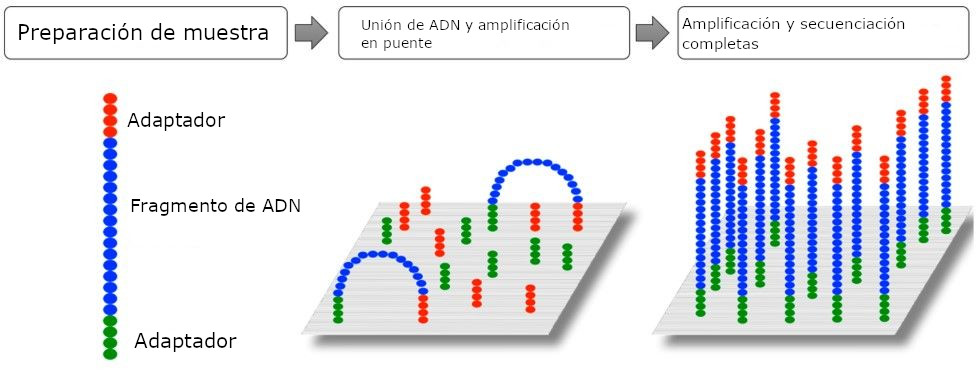
\includegraphics[width=14.1cm]{figuras/IMG_3}
\caption*{\textbf{Figura 3.-} Amplificación de PCR en puente y clústeres de librerías de ADN (Tomada y modificada de: \cite{Garrido-Cardenas2017}.)}
\label{Figura 3}
\end{figure}
\\[30cm]
\begin{figure}[!h]
\addcontentsline{lof}{section}{\textbf{Figura 4.-} Secuenciación de librerías mediante fluorescencia.}
\centering
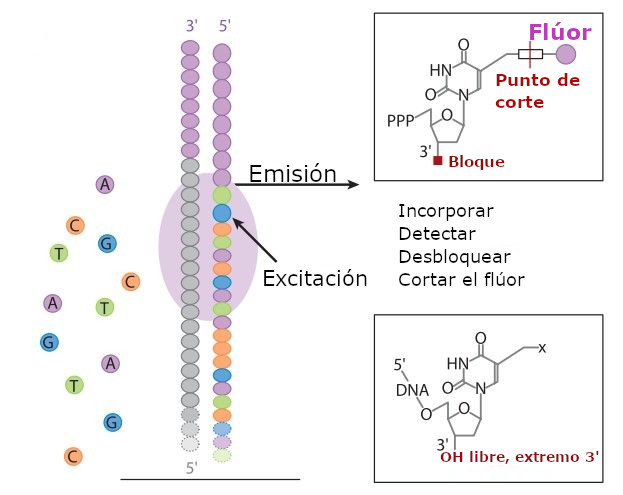
\includegraphics[width=10.11cm]{figuras/IMG_4}
\caption*{\textbf{Figura 4.-} Secuenciación de librerías mediante fluorescencia (Tomada y modificada de: \cite{Mardis2013}.)}
\label{Figura 4}
\end{figure}

\subsection{Secuenciación de ADN del marcador 16S ARNr}
En metagenómica existen dos clases de secuenciación: shotgun y secuenciación por amplicones. No obstante, el segundo tipo de secuenciación tiene la ventaja de que se requieren menos secuencias para caracterizar una muestra, por lo que resulta más barata en comparación con el otro. Este tipo de secuenciación se basa en el uso de marcadores genéticos, y el más utilizado para bacterias es el 16S, el cual posee tanto regiones altamente conservadas (utilizadas para diseñar iniciadores) así como regiones que son hipervariables (para identificar características filogenéticas). En este sentido, la región V4 del gen 16S es una región hipervariable semiconservada, que da una lectura más precisa a nivel taxonómico filo, pero permite la identificación de microorganismos incluso hasta nivel de género. Además, el análisis de datos presenta una metodología más estandarizada. Debido a esto, la mayoría de estudios optan por este camino a la hora de identificar comunidades microbianas; aunque aún es necesario mejorar este método porque presenta diversos sesgos, por ello es considerado como un análisis semicuantitativo \autocite{Ranjan2016,Sanschagrin2014,Yang2016}.
\section{Análisis bioinformáticos}
La bioinformática es una disciplina que combina la biología y la informática para interpretar datos biológicos. Los investigadores desarrollan códigos de programación que se adecuen a determinadas necesidades, ya sea para el análisis de secuencias de datos, predicción de genes, modelado de proteínas entre otros. Para obtener lecturas que sean relevantes, se tiene que realizar un procesado de los datos crudos que se obtienen de la secuenciación, esto con la finalidad de tener una mayor calidad en los datos \autocite{Lesk2019}.
\par
Los pasos generales a seguir son:
\begin{itemize}
\item Alineación de secuencias
\item Filtro de calidad 
\item Eliminación de secuencias quiméricas
\end{itemize}
\subsection{Formato de archivos de secuenciación}
En la secuenciación por síntesis, el instrumento detecta cada una de las bases de cada hebra de ADN, así como de su código de barras correspondiente, y genera un archivo tipo fastq. De acuerdo con la intensidad de la señal fluorescente detectada para cada base, y a la intensidad de fluorescencia correspondiente a otras bases (intensidad de fluorescencia de fondo), el secuenciador asigna también una calidad a cada base. La calidad se mide en la escala Phred, donde la probabilidad de una base errónea (p) se expresa logarítmicamente, mediante la siguiente formula \autocite{Cock2009}.
\begin{large}
 \[Phred=-10log_{10}(p)\]
\end{large}
Por ejemplo, un valor de Phred 10 corresponde a una probabilidad 1:10 de una base incorrecta, mientras que un valor Phred 30 corresponde a 1:1000. Para representar la calidad de una base con un sólo dígito, se utiliza el código ASCII. En instrumentos Illumina actuales, la escala va de ! a K, correspondiente a 0 a 42 Phred. Los archivos fastq son de texto plano. Si se utiliza secuenciación tipo “paired-end”, cada hebra se secuenciará en dos direcciones, forward y reverse. En ese caso, se obtendrá un archivo fastq independiente para las secuencias forward y reverse. El formato fastq contiene cuatro líneas para cada lectura \autocite{Cock2009}:
\par 
Línea 1: @Nombre o ID de la secuencia. Siempre empieza con @ y puede tener información sobre la muestra, la corrida, etc.
\par
Línea 2: Secuencia. Contiene los caracteres A, G, C, T, así como caracteres para bases ambiguas, como N o R, Y, S, W, K, M, B, D, H y V
\par
Línea 3: +
\par
Línea 4: Calidad en Código Phred. 
Por ejemplo, esta es una secuencia obtenida en el presente estudio: 
\par
@M03776:117:000000000-B554V:1:1101:16180:1493 1:N:0:0
\begin{sloppypar}
CTACCCTCCCGACTGCCTATGCTGTTTATCCTTTGGATGGTCGCCATGATGGTGGTT
ATTATACCGTCAAGGACTGTGTGACTATTTACGTCCTTCCCCGTACGCCGGGCAATA
ATGTTTATGTTGGTTTCATGGTTTGGTCTAACTTTACCGCTACTAAATGCCGCGGATT
GGTTTCGCTGAATCAGGTTATTAAAGAGATTATTTGTCTCCAGCCACTTAATGATCG
GAAGAGCGGTTCAGCAGGAATG
\end{sloppypar}
+
\begin{sloppypar}
\textbf{1\textgreater 1\textgreater 1BDA\textgreater \textgreater 11AA10AB1BF1BADFF3DAAFGGB01B10BF?/A/BC1DA1F1/BFBGHGF
DE2/FE//B10\textgreater B/F1GA1DFBDG22@/GC\textgreater EGE0B\textgreater /?/?//\textgreater ///\textless //B11B\textgreater FGG2F2GG2/
?FGG2F21FFG//??F11?FGH11\textless /-A-\textless \textgreater 111\textgreater 1\textless \textless \textless ----:AG.CGHF?.C..00;000;F0;
F000;0//;C0CFF0CBFB00//-9-;F///9/;9--------9-A=9////9---;/}
\end{sloppypar}
\newpage
\subsection{Software de análisis}
Existen diversos paquetes bioinformáticos que son utilizados para el proceso y análisis de información biológica, muchos de estos programas requieren de habilidades en informática para ejecutarlos de manera correcta. Diversas empresas ponen a disposición su propio software para el análisis de datos, sin embargo, los costos de estos programas suelen elevarse. Por ello existen paquetes que son de código abierto, a los cuales cualquier persona puede acceder a ellos sin ningún costo \autocite{Almeida2019,Upadhyayula2019}.
\subsubsection{QIIME 2}
Quantitative Insights Into Microbial Ecology, es un software que desarrolló \textcite{Caporaso2010a}. Se caracteriza por estar programado en Python y ser de código abierto. En su versión más actual (2019.1), importa datos crudos de la secuenciación, demultiplexea los datos, remueve datos innecesarios, filtra por calidad y asigna a una taxonomía, analiza los datos y obtiene información.
\subsubsection{PICRUSt}
Phylogenetic Investigation of Communities by Reconstruction of Unobserved States. Este software se encarga de predecir el contenido funcional del metagenóma usando un algoritmo de reconstrucción ancestral que predice las familias presentes para posteriormente combinarlas y así estimar la composición del metagenóma. Se apoya a partir de los datos obtenidos del gen marcador 16S ARNr y de una base de datos de genomas. Su principio es que los microorganismos con alta similitud en el gen 16S ribosomal, tienen muchas veces genomas similares. Entonces, si se comparan las secuencias de 16S con las de los genomas disponibles, y se localizan los genomas más similares para cada 16S de una muestra ambiental, se pueden predecir los genes presentes en este ambiente con bastante éxito \autocite{Langille2013}.
\par
Este método tiene algunas limitaciones. Por un lado, existen muchos microorganismos para los que no se tienen genomas en las bases de datos. Los genes de estos microorganismos no se pueden predecir utilizando PICRUSt y suelen tener, además del genoma núcleo, un genoma accesorio \autocite{Alcaraz2010}. El genoma núcleo se encuentra por definición en todos los microorganismos de una especie, mientras que el genoma accesorio puede variar entre distintas cepas. Por lo tanto, al detectar el 16S de una cepa en el ambiente, las predicciones sobre la presencia de genes del genoma núcleo son robustas, mientras que las del genoma accesorio están sujetas a mayor incertidumbre. En general, se desconoce cuáles genes pertenecen al genoma núcleo y cuáles al genoma accesorio. Entre más genomas cercanos hay en las bases de datos para cada secuencia de 16S, hay mayor probabilidad de predecir correctamente genes del genoma accesorio \autocite{Langille2013}.
\section{Biodiversidad microbiana}
La biodiversidad o diversidad biológica, es la variabilidad de organismos que se encuentran en los diferentes niveles de organización, como los sistemas terrestres y acuáticos. Puede ser clasificada en tres grandes categorías, diversidad alfa, diversidad beta y diversidad gamma \autocite{Magurran2013,Tuomisto2010a}.
\subsection{Diversidad Gamma}
La diversidad gamma es la más sencilla de definir: son todas las especies efectivas que se encuentran en un ambiente. Por ejemplo, supongamos que una misma especie se encuentra localizada en varias regiones, y están separadas a cierta distancia entre sí, entonces todos los organismos que pertenezcan a la misma especie, aunque estén separados pertenecerán a la diversidad gamma \autocite{Hunter2007}. Esta diversidad se puede dividir en dos: alfa y beta.
\newpage
\subsection{Diversidad Alfa}
Es la media de especies a una escala local, donde por ejemplo se encuentran dos organismos que pertenecen a la misma especie, pero tienen características diferentes. Esta diversidad puede cuantificarse directamente de los datos obtenidos, su particularidad es que esta clasificación se hace de cada una de las sub unidades por separado. Para determinar la diversidad alfa se ocupan distintos índices, como el índice de Simpson y el índice de Shannon, así como la curva de rarefacción \autocite{Tuomisto2010}.
\subsubsection{Índice de Simpson}
El índice de Simpson es una ecuación matemática que determina la probabilidad de que dos individuos obtenidos al azar de una comunidad, pertenezcan a la misma especie. Donde la proporción de especies \(i\) en relación con el número total de las mismas \(pi\) es calculado y se ajusta al cuadrado para el total de ellas \autocite{Tuomisto2010}. 
\begin{large}
 \[\lambda=\sum p_i^{2}\]
\end{large}
Donde \(p_i\) es igual a la proporción de individuos de la especie \(i\). Así, mientras \(\lambda\) incrementa, la diversidad disminuye, por ello el índice de Simpson es usualmente expresado como \(D= 1/\lambda\).
\subsubsection{Índice de Shannon}
El índice de Shannon supone que: todos los individuos de una comunidad se muestrean aleatoriamente y que todas las especies son representadas dentro de la muestra. Se expresa en la ecuación donde: la proporción de especies \(i\) en relación al número total de especies \(pi\) es calculado, posteriormente es multiplicada por el logaritmo natural de esta proporción, luego el resultado es sumado entre las especies y multiplicado por -1. De igual manera, considera el grado de uniformidad y la abundancia de especies. El índice de Shannon viene de la teoría de la información, y cuantifica, en bits, cuánta información se requiere para describir una comunidad. Entre más compleja, es decir, con más variedad de microorganismos, y alta predominancia de muchas especies, una comunidad requiere más bits para ser descrita, y es por lo tanto más biodiversa \autocite{Tuomisto2010a}.
\begin{large}
\[H'=\sum p_i ln p_i\]
\end{large}
\subsubsection{Curva de rarefacción}
La curva de rarefacción es una representación gráfica de las especies observadas de cada una de las muestras analizadas (Fig. 5), que usualmente es utilizada en análisis de especies, unidades taxonómicas operativas (OTU) u otra unidad que describa grupos biológicos de interés. La curva de rarefacción permite comparar la diversidad alfa de muestras con diferente número de observaciones (por ejemplo, diferente número de lecturas de secuencias de 16S). Básicamente, mide el número de especies encontrada por muestra o por lectura. Se obtiene tomando sub-muestras aleatorias de la muestra original incrementando gradualmente el tamaño sub-muestreado. Con sub-muestras pequeñas, se obtiene una diversidad baja, que va aumentando linealmente conforme se aumenta el tamaño de la sub-muestra. Es decir, al considerar más observaciones se "descubren" nuevos organismos presentes en la muestra original. Sin embargo, al tomar muestras mayores, estas tienden a contener más organismos repetidos, por lo que el incremento deja de ser lineal, y la curva se aplana, acercándose a una asíntota. Esta asíntota representa la diversidad real de la comunidad. Entonces, uno de los objetivos principales de las curvas de rarefacción es determinar si se han hecho suficientes observaciones (por ejemplo, lecturas de secuenciación) para realizar una estimación de la diversidad de la comunidad con suficiente confiabilidad \autocite{Siegel2006}.
\begin{figure}[h]
\addcontentsline{lof}{section}{\textbf{Figura 5.-} Representación de una curva de rarefacción.}
\centering
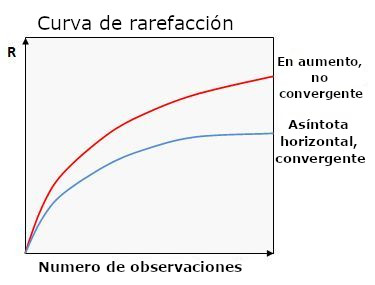
\includegraphics[width=7cm]{figuras/IMG_5}
\caption*{\textbf{Figura 5.-} Representación de una curva de rarefacción (Tomada y modificada de: \cite{Edgar2018}.}
\label{Figura 5}
\end{figure}
\subsection{Diversidad Beta}
Mientras que la diversidad alfa mide la diversidad local, por ejemplo, en una muestra de una comunidad microbiana, la diversidad beta refleja el cambio de la biodiversidad a través del tiempo o el espacio. Es decir, compara diferentes comunidades locales, o una misma comunidad en el tiempo. En esencia compara dos muestras, donde toma en cuenta las similitudes y diferencias que hay entre ellas. De igual manera existen distintos índices para medir la diversidad Beta, por ejemplo: índice de Bray-Curtis, distancia Euclidiana y la distancia UniFrac, entre otros \autocite{Tuomisto2010a}.
\chapter{Justificación}
En la actualidad, México enfrenta diversos problemas en la producción de alimentos y en especial en maíz, ya que una gran parte del cereal que se consume en el país se importa de Estados Unidos. Derivado de esto, se han planteado diversas soluciones para aumentar la producción y el rendimiento de los cultivos, así como la reducción del uso de agroquímicos. Las milpas que son cultivadas en la región del Alto Mezquital se caracterizan porque conservan las técnicas de antaño para su labranza, por lo que no intervienen agentes químicos añadidos, y además existe una alta diversidad de cultivos en una misma parcela que permite que el suelo este exento de condiciones que lo erosionen. Estas características son ideales, debido a que las comunidades bacterianas que habitan en el suelo no se ven alteradas por cambios químicos artificiales que pudieran repercutir en su composición y en las interacciones que tienen con los cultivos. Estas comunidades son de importancia por su relación simbiótica con las plantas, puesto que existe un intercambio de nutrientes entre ambos, además de otras interacciones benéficas, como la estimulación del crecimiento vegetal por fitohormonas producidas por los microorganismos, y la supresión de microorganismos fitopatógenos. Por ello, identificar las funciones metabólicas que desempeñan las comunidades bacterianas permitirá desarrollar técnicas de agricultura sustentable, tales como la elaboración de biofertilizantes, bioinsecticidas entre otros.
\chapter{Hipótesis}
Las milpas tradicionales son agroecosistemas que no han sido impactadas por el uso de insumos agrícolas químicos en donde conviven varios tipos de cultivos siendo el maíz el principal, por lo tanto, la microbiota asociada a sus suelos posee comunidades microbianas particulares con funciones metabólicas específicas que son enriquecidas por las raíces de éste cereal.
\chapter{Objetivos}
\section{Objetivo general}
Analizar las comunidades bacterianas en los suelos de una milpa de la localidad El Boxo municipio de Cardonal en el estado de Hidalgo, mediante metagenómica y software especializado para predecir las funciones metabólicas que intervienen en este agroecosistema.
\section{Objetivos específicos}
\begin{itemize}
\item Determinar la estructura de las comunidades bacterianas del suelo de milpa, mediante estudios de metagenómica, para la comparación de los suelos que presentan influencia por las raíces de maíz con aquellos que no la tienen.
\item Analizar las comunidades microbianas asociadas a los suelos de la milpa con y sin la influencia de las raíces de maíz para determinar las diferencias en las funciones metabólicas que desempeñan mediante el uso de software especializado, técnicas de visualización de datos, así como análisis estadísticos. 
\end{itemize}
\chapter{Metodología}
\section{Área de estudio}
La primera fase que se llevó a cabo en este proyecto fue la ubicación de la milpa, ésta, se encuentra en la comunidad de El Boxo ($\SI{20}{\degree}$ 40' 38.8'' N $\SI{99}{\degree}$ 08' 43.0'' W) perteneciente al municipio de El Cardonal, en la región geográfica denominada como El Alto Mezquital, Estado de Hidalgo (Fig. 6 y 7).
%\begin{figure}[!h]
%\addcontentsline{lof}{section}{\textbf{Figura 6.-} Mapa geográfico del estado de Hidalgo.}
%\centering
%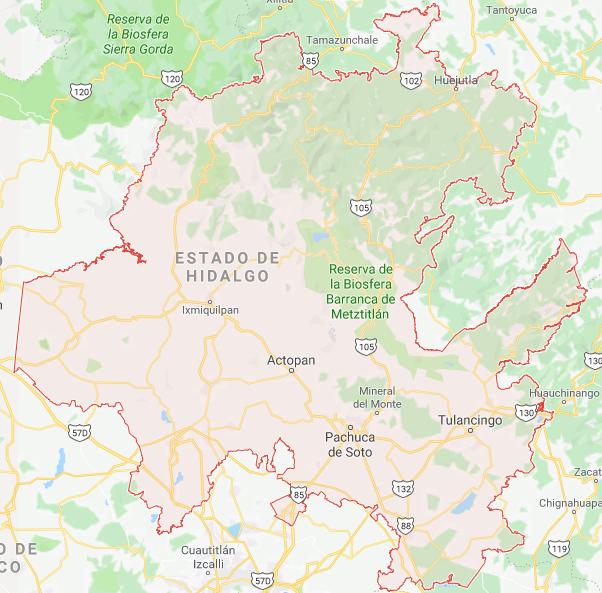
\includegraphics[width=11.95cm]{figuras/IMG_6}
%\caption*{\textbf{Figura 6.-} Mapa geográfico del estado de Hidalgo, se muestran algunos de los municipios más importantes.}
%\label{Figura 6}
%\end{figure}
\begin{figure}[!h]
\addcontentsline{lof}{section}{\textbf{Figura 6.-} Ubicación de la comunidad de El Boxo.}
\centering
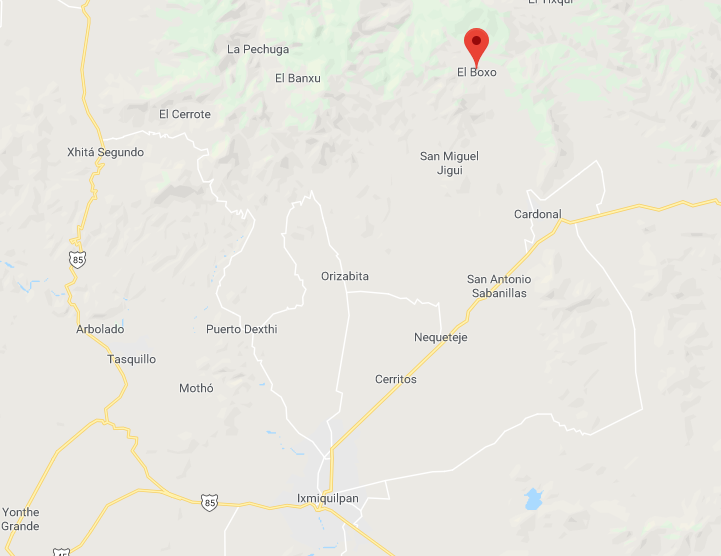
\includegraphics[width=14.13cm]{figuras/IMG_7}
\caption*{\textbf{Figura 6.-} Ubicación de la comunidad de El Boxo, se encuentra aproximadamente a 30 km de la cabecera municipal de Ixmiquilpan.}
\label{Figura 7}
\end{figure}
\begin{figure}[!h]
\addcontentsline{lof}{section}{\textbf{Figura 7.-} Ubicación exacta del área de estudio.}
\centering
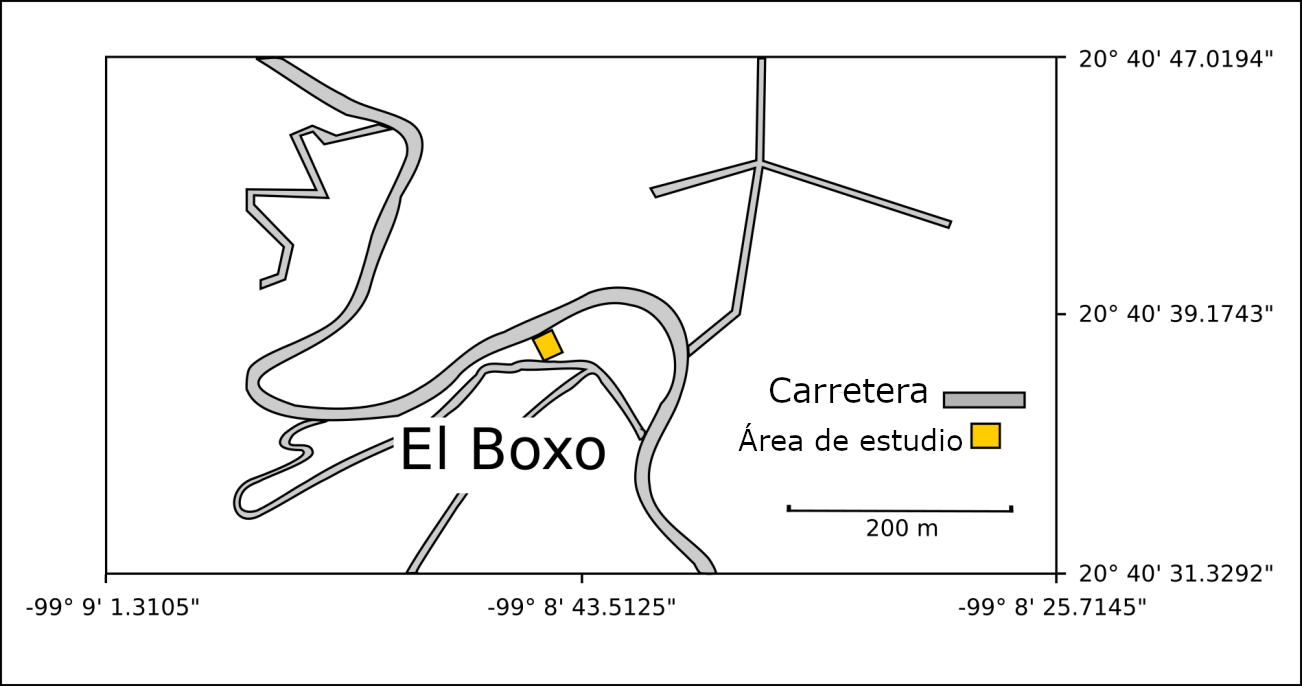
\includegraphics[width=15.03cm]{figuras/IMG_8}
\caption*{\textbf{Figura 7.-} Ubicación exacta del área de estudio.}
\label{Figura 8}
\end{figure}
\section{Muestreo}
El muestreo se realizó en diciembre de 2016, en plantas de maíz maduras ya con mazorcas, sembradas a intervalos regulares, con una distancia de 100 cm de distancia entre surcos. Se seleccionaron 6 plantas aleatoriamente para el muestreo, evitando las de la orilla de la parcela ya que alrededor se encontraban árboles frutales  que podrían ocasionar sesgos en el muestreo. La colecta de suelo se realizó utilizando una bayoneta, la cual fue lavada y desinfectada con alcohol antes de tomar cada muestra. Con este instrumento, se obtuvieron núcleos de suelo de 20 a 30 cm de profundidad. Utilizando guantes de látex, se colectó un segmento del núcleo, correspondiente a una profundidad aproximada de 10 cm, evitando colectar rocas o fragmentos visibles de raíz.  Las muestras se guardaron en bolsas estériles de polipropileno, y se colocaron en nitrógeno líquido para su transporte al laboratorio. Una vez en el laboratorio, las muestras se almacenaron en un ultracongelador, a aproximadamente  $\SI{-70}{\degreeCelsius}$.
\par
Se colectaron dos tipos de muestras. Para determinar la influencia de las raíces de plantas de maíz en el microbioma del suelo, se tomaron los suelos adyacentes a las plantas seleccionadas. Estas muestras se rotularon con la letra M, seguidas por números secuenciales, del 1 al 6, para identificar cada planta. Como control, se colectaron muestras representativas del suelo de la milpa, a una distancia de 30 cm de cada planta muestreada, evitando la presencia de otras plantas en estos puntos. Estas muestras se rotularon con una letra C, y el número correspondiente a la planta más cercana.
\section{Análisis del suelo}
Para el análisis del suelo, las muestras se recolectaron utilizando una pala, y fueron colocadas en bolsas limpias. Estas muestras fueron enviadas al Centro de Investigación en Alimentación y Desarrollo, A.C., donde fueron analizadas mediante la norma NOM-021-RECNAT-2000, para determinar el tamaño de partícula, pH, materia orgánica y nutrientes.
\section{Extracción de ADN}
Se extrajo ADN total de cada una de las muestras, correspondiente a toda la comunidad bacteriana del suelo presente en cada punto de muestreo. Para tal efecto, se utilizó el kit Power soil isolation (MoBio, Carlsbad, CA, USA), siguiendo las instrucciones que el fabricante recomendaba. El procedimiento de extracción inició con una lisis mecánica y química, y posteriormente el ADN se capturó en una membrana de sílice. Se realizó una serie de lavados para eliminar contaminantes e inhibidores de la Reacción en Cadena de la Polimerasa (PCR por sus siglas en inglés) presentes en suelos. Los ácidos nucleicos obtenidos de la extracción, se colocaron en 12 tubos Eppendorf, correspondientes a las muestras y sus controles, los cuales se almacenaron en un congelador (aproximadamente $\SI{-20}{\degreeCelsius}$).
\newpage
\section{Secuenciación de ADN}
La secuenciación del ADN obtenido de muestras de suelo de la milpa estudiada se realizó en colaboración con el Dr. Jorge Rocha-Estrada, en el laboratorio del Dr. Roberto Kolter, de la Universidad de Harvard; en un secuenciador Illumina MiSeq.
\par
Previamente a la secuenciación, se prepararon librerías a partir del ADN genómico que consistió en amplificar el fragmento de interés, utilizando los iniciadores F515 (5’ – GTGCCAGCMGCCGCGGTAA – 3’) y R806 (5’ – GGACTACHVGGGTWTCTAAT – 3’) específicos para la región V4 del gen 16S ARNr \autocite{Caporaso2010b}.
\par
Adicionalmente, a los iniciadores, tanto directo como reverso, se les agregaron secuencias requeridas para la secuenciación. Las cuales se incorporaron al producto de PCR en el primer ciclo de amplificación, quedando ligadas al producto final. Los iniciadores directos utilizados contienen:
\par
1.- Adaptador Illumina 5'. Esta secuencia es complementaria a las hebras de ADN fijas a la celda de Illumina, y permiten la amplificación por puentes.
\par
2.- Iniciador directo pad. Esta secuencia separa al adaptador de la secuencia linker, y ayuda a evitar estructuras secundarias que podrían obstaculizar la reacción de PCR.
\par
3.- Iniciador directo linker. Esta secuencia es complementaria a una región equivalente en la secuencia reversa. Sirve para asegurar la amplificación del adaptador y del código de barras. 
\par
4.- Iniciador directo. Este es el iniciador de la región biológica de interés, en este caso la región V4 del gen 16S que tiene aproximadamente 251pb.
\par
Los iniciadores reversos utilizados tuvieron una estructura muy similar, con la excepción que en el adaptador Illumina y el iniciador pad se insertó un código de barras, diferente para cada una de las muestras. Estos códigos de barras permitieron identificar de qué muestra provino cada secuencia obtenida. Una vez preparadas las librerías, se procedió a la secuenciación por puentes en el instrumento MiSeq, del cual se obtuvieron los archivos fastq con las secuencias, para su análisis \autocite{Fadrosh2014}.

\section{Análisis bioinformático}
\subsection{Análisis en QIIME 2}
Los archivos obtenidos del secuenciador se procesaron con la plataforma bioinformática QIIME 2 (versión 2019.1). El procesamiento de los datos consistió en los siguientes pasos:
\begin{itemize}
\item Se separaron las lecturas por muestra. Debido a que las secuencias se encontraban en un solo par de archivos fastq, se utilizó la información del código de barras de cada lectura, para separarlas de acuerdo con el número de muestra a la que corresponden (En inglés, este paso se conoce como Demultiplexing).
\item Limpieza y ensamblado. Las lecturas fueron limpiadas, eliminando las partes que tuvieron calidad deficiente, de acuerdo con su valor Phred. Las secuencias limpias se ensamblaron, juntando las lecturas forward y reverse. Asimismo, en este paso se filtraron las secuencias quiméricas mediante el algoritmo DADA2, en QIIME \autocite{Callahan2016}.
\item Tabla de abundancias y clasificación taxonómica. Las secuencias limpias y libres de quimeras se utilizaron para crear una tabla de las abundancias relativas de los microorganismos, donde para cada secuencia se cuantificó la presencia correspondiente en cada muestra. Estas secuencias se clasificaron taxonómicamente, utilizando un clasificador bayesiano \autocite{Werner2011}, entrenado con la base de datos Green Genes \autocite{DeSantis2006}. De esta manera, se logró la clasificación de las bacterias de la comunidad a nivel de filo, clase, orden, familia, y género, siempre que fue posible. La tabla generada fue la base para diferentes análisis, incluyendo comparaciones entre las muestras correspondientes a los suelos cercanos alejados de las raíces \autocite{Aguirre-von-Wobeser2018}. En este trabajo, se infirió a partir de dicha tabla de abundancias, las rutas metabólicas presentes en los distintos grupos de muestras, asociadas a las raíces del maíz, y controles de suelo.
\end{itemize}
\subsection{Predicción de rutas metabólicas}
Para comprender mejor los procesos involucrados en el suelo, en particular las posibles funciones de los microorganismos en suelo adyacente a las raíces de maíz, se realizó una predicción de las rutas metabólicas presentes en este ambiente. Para este fin, se utilizó PICRUSt el cual es un software que utiliza algoritmos para predecir genes de rutas metabólicas que podrían estar involucradas en los procesos del suelo. Las predicciones de PICRUSt se basan en comparar las secuencias de 16S de los organismos detectados, con una base de datos de genomas completos. De esta manera, si una ruta metabólica se encuentra presente en determinado genoma, se predice su presencia en el ambiente que contengan dicho genoma, de acuerdo con el 16S \autocite{Langille2013}. 
\par
El procedimiento utilizado para el análisis mediante PICRUSt se resume de la siguiente manera:
\begin{itemize}
\item La tabla de abundancias obtenida de QIIME 2 que contenía un agrupamiento de OTU's closed reference, en formato biom, sirvió como entrada para el programa PICRUSt. Para este análisis, se utilizó la plataforma Galaxy (http://galaxy.morganlan\\gille.com/), que realiza el análisis en línea.
\item El número de copias del gen 16S puede variar en diferentes bacterias. Debido a ello, se normalizó por el número de copias de 16S presentes en los genomas de referencia.
\item Con la tabla de abundancias normalizada, se realizó la predicción del metagenóma, tomando la base de datos Green Genes \autocite{DeSantis2006} como referencia para la tabla de abundancias. Se configuró el análisis para predecir genes de las rutas metabólicas de la base de datos Kyoto Encyclopedia of Genes and Genomes (KEGG) \autocite{Kanehisa2000}. Mediante este análisis, se obtuvo una tabla de abundancias predichas para los diferentes genes predichos, de acuerdo con su ID de KEGG.
\end{itemize}
\subsection{Análisis estadístico}
De los datos que se obtuvieron en PICRUSt se procesaron en el software estadístico R. Las predicciones de las rutas metabólicas para las muestras de suelo tomadas en las raíces de las plantas de maíz se compararon con las predicciones para el suelo libre de raíces. Para este fin, se utilizó una prueba no paramétrica de Wilcoxon para cada gen, al 95\% de confianza (p\textless 0.05).
\par 
Los genes que presentaron diferencias significativas entre las comunidades de las raíces de las plantas de maíz, con respecto a los controles, se localizaron en mapas de las rutas metabólicas de KEGG, utilizando el software KEGG Mapper \autocite{Kanehisa2019}. Esto permitió predecir qué procesos se realizan favorablemente en las comunidades microbianas influenciadas directamente por las plantas de maíz.
 
\chapter{Resultados y Discusión}
\section{Análisis fisicoquímico del suelo}
De acuerdo al análisis fisicoquímico realizado al suelo de El Boxo (Tabla 5), éste se caracteriza por tener una textura franco-arcillosa. Su pH de 6.7, permite que el suelo sea neutro, por lo que es ideal para la agricultura. Como determinan \textcite{Zhalnina2014}, el pH del suelo influye en la composición microbiana, debido a que funge como un mediador que pone a disposición los nutrientes requeridos para las bacterias.
%\begin{table}[!ht]
\addcontentsline{lot}{section}{\textbf{Tabla 5.-} Parámetros fisicoquímicos que componen el suelo de la milpa de El Boxo.}
%\centering
%\caption*{\textbf{Tabla 5.-} Parámetros fisicoquímicos que componen el suelo de la milpa de El Boxo.}
%\label{Tabla 5}
\begin{longtable}[c]{cc}
%\centering
\caption*{\textbf{Tabla 5.-} Parámetros fisicoquímicos que componen el suelo de la milpa de El Boxo.} \label{Tabla 5} \\
\toprule[0.5mm]
\multicolumn{2}{c}{Parámetros fisicoquímicos} \\
\midrule
Arena & 29\% \\ 
Arcilla & 39\% \\ 
Limo & 32\% \\ 
Materia orgánica & 3.61\% \\ 
pH & 6.7 \\ 
\ce{N-NO3} & 47.4 ppm \\ 
\ce{P-PO4} & 196.6 ppm \\ 
\ce{K} & 289 ppm \\ 
\ce{Ca} & 7680 ppm \\ 
\ce{Mg} & 570 ppm \\ 
\ce{S} & 20 ppm \\ 
\ce{Fe} & 8.8 ppm \\ 
\ce{Cu} & 2.2 ppm \\ 
\ce{Zn} & 11 ppm \\ 
\ce{Mn} & 5.5 ppm \\ 
\ce{Na} & 92 ppm \\ 
\bottomrule[0.5mm]
\end{longtable}
\par
\textcite{Beales2004} explica que, si el pH del suelo es ácido, entonces la actividad enzimática de las bacterias se inhibe provocando que una menor cantidad de ellas que no son tolerantes a esta condición, mueran. Sin embargo, existen bacterias que a lo largo de los años han desarrollado resistencia a ambientes ácidos \autocite{Dilworth2001}. Derivado de esto, un suelo que es enriquecido con fertilizantes con base de amonio alterará el pH drásticamente, provocando una disminución de las comunidades bacterianas que habiten en el ecosistema \autocite{Zeng2016}. Probablemente, la nula utilización de agroquímicos en la milpa estudiada favorece el pH neutro.
\par
El suelo de la milpa es rico en nutrientes, lo que también favorece el crecimiento de las plantas. De acuerdo con el análisis fisicoquímico que se realizó al suelo de la milpa, este contiene exceso de nitratos y fosfatos, así como concentraciones altas de sulfato, potasio, magnesio, cobre y zinc.
\par
\section{Extracción de ADN}
Para análisis de las comunidades microbianas del suelo de la milpa de El Boxo, se realizaron las extracciones de ADN de cada una de las muestras. Se cuantificó su concentración, para determinar si cubrían los requerimientos mínimos para efectuar el protocolo de Illumina Miseq (Fig. 8).
\newpage
Con excepción de la muestra 4C, correspondiente al control de la planta 4, se obtuvieron concentraciones apropiadas para la amplificación de la región V4 del gen 16S, y su posterior secuenciación. 
\begin{figure}[!h]
\addcontentsline{lof}{section}{\textbf{Figura 8.-} Concentraciones de ADN de cada muestra.}
\centering
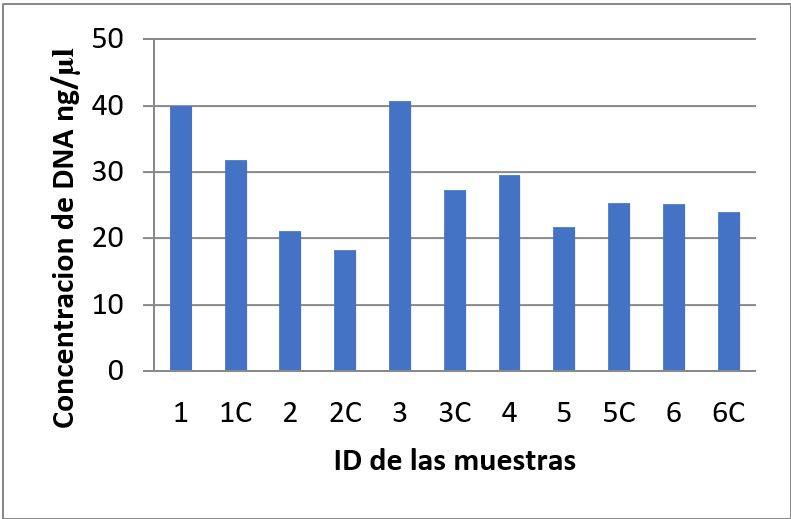
\includegraphics[width=10cm]{figuras/IMG_9}
\caption*{\textbf{Figura 8.-} Concentraciones de ADN extraído de muestras de suelo colectadas en una milpa de El Boxo municipio de Cardonal en el estado de Hidalgo. El ID de las muestras indica el número de planta muestreada, y la C indica las muestras correspondientes a los controles cercanos a cada planta (a 30 cm de distancia).}
\label{Figura 9}
\end{figure}
\section{Análisis de secuencias}
Después de la secuenciación, los datos crudos obtenidos se procesaron en QIIME 2, obteniendo 554,745 lecturas de la demultiplexación. Para la purificación de las secuencias se utilizó el comando DADA2. Posteriormente se determinó el filo al que pertenecian las secuencias y se encontró una mayor presencia \textit{Proteobacteria, Acidobacteria, Actinobacteria, Bacteroidetes, Chloroflexi, Planctomycetes, Verrucomicrobia y Gemmatimonadetes} (Fig. 9).
\par
Diversos autores reportan que \textit{Proteobacteria} es el filo más común en el suelo \autocite{Buckley2003,Janssen2006}, seguido por el filo \textit{Acidobacteria}, tal como se comprobó en este trabajo. Comparando  las muestras de las raíces  con los controles, en este proyecto se encontró que la proporción de representantes de los filos \textit{Actinobacteria} y \textit{Verrucomicrobia}, así como del orden \textit{Burkholderiales} era mayor en el suelo de la rizosfera que en el suelo libre de raíces como lo mencionan \autocite{Aguirre-von-Wobeser2018}. %poner esta cita sin parentesis
\begin{figure}[!h]
\addcontentsline{lof}{section}{\textbf{Figura 9.-} Abundancia relativa del filo de bacterias en suelos de la milpa de El Boxo.}
\centering
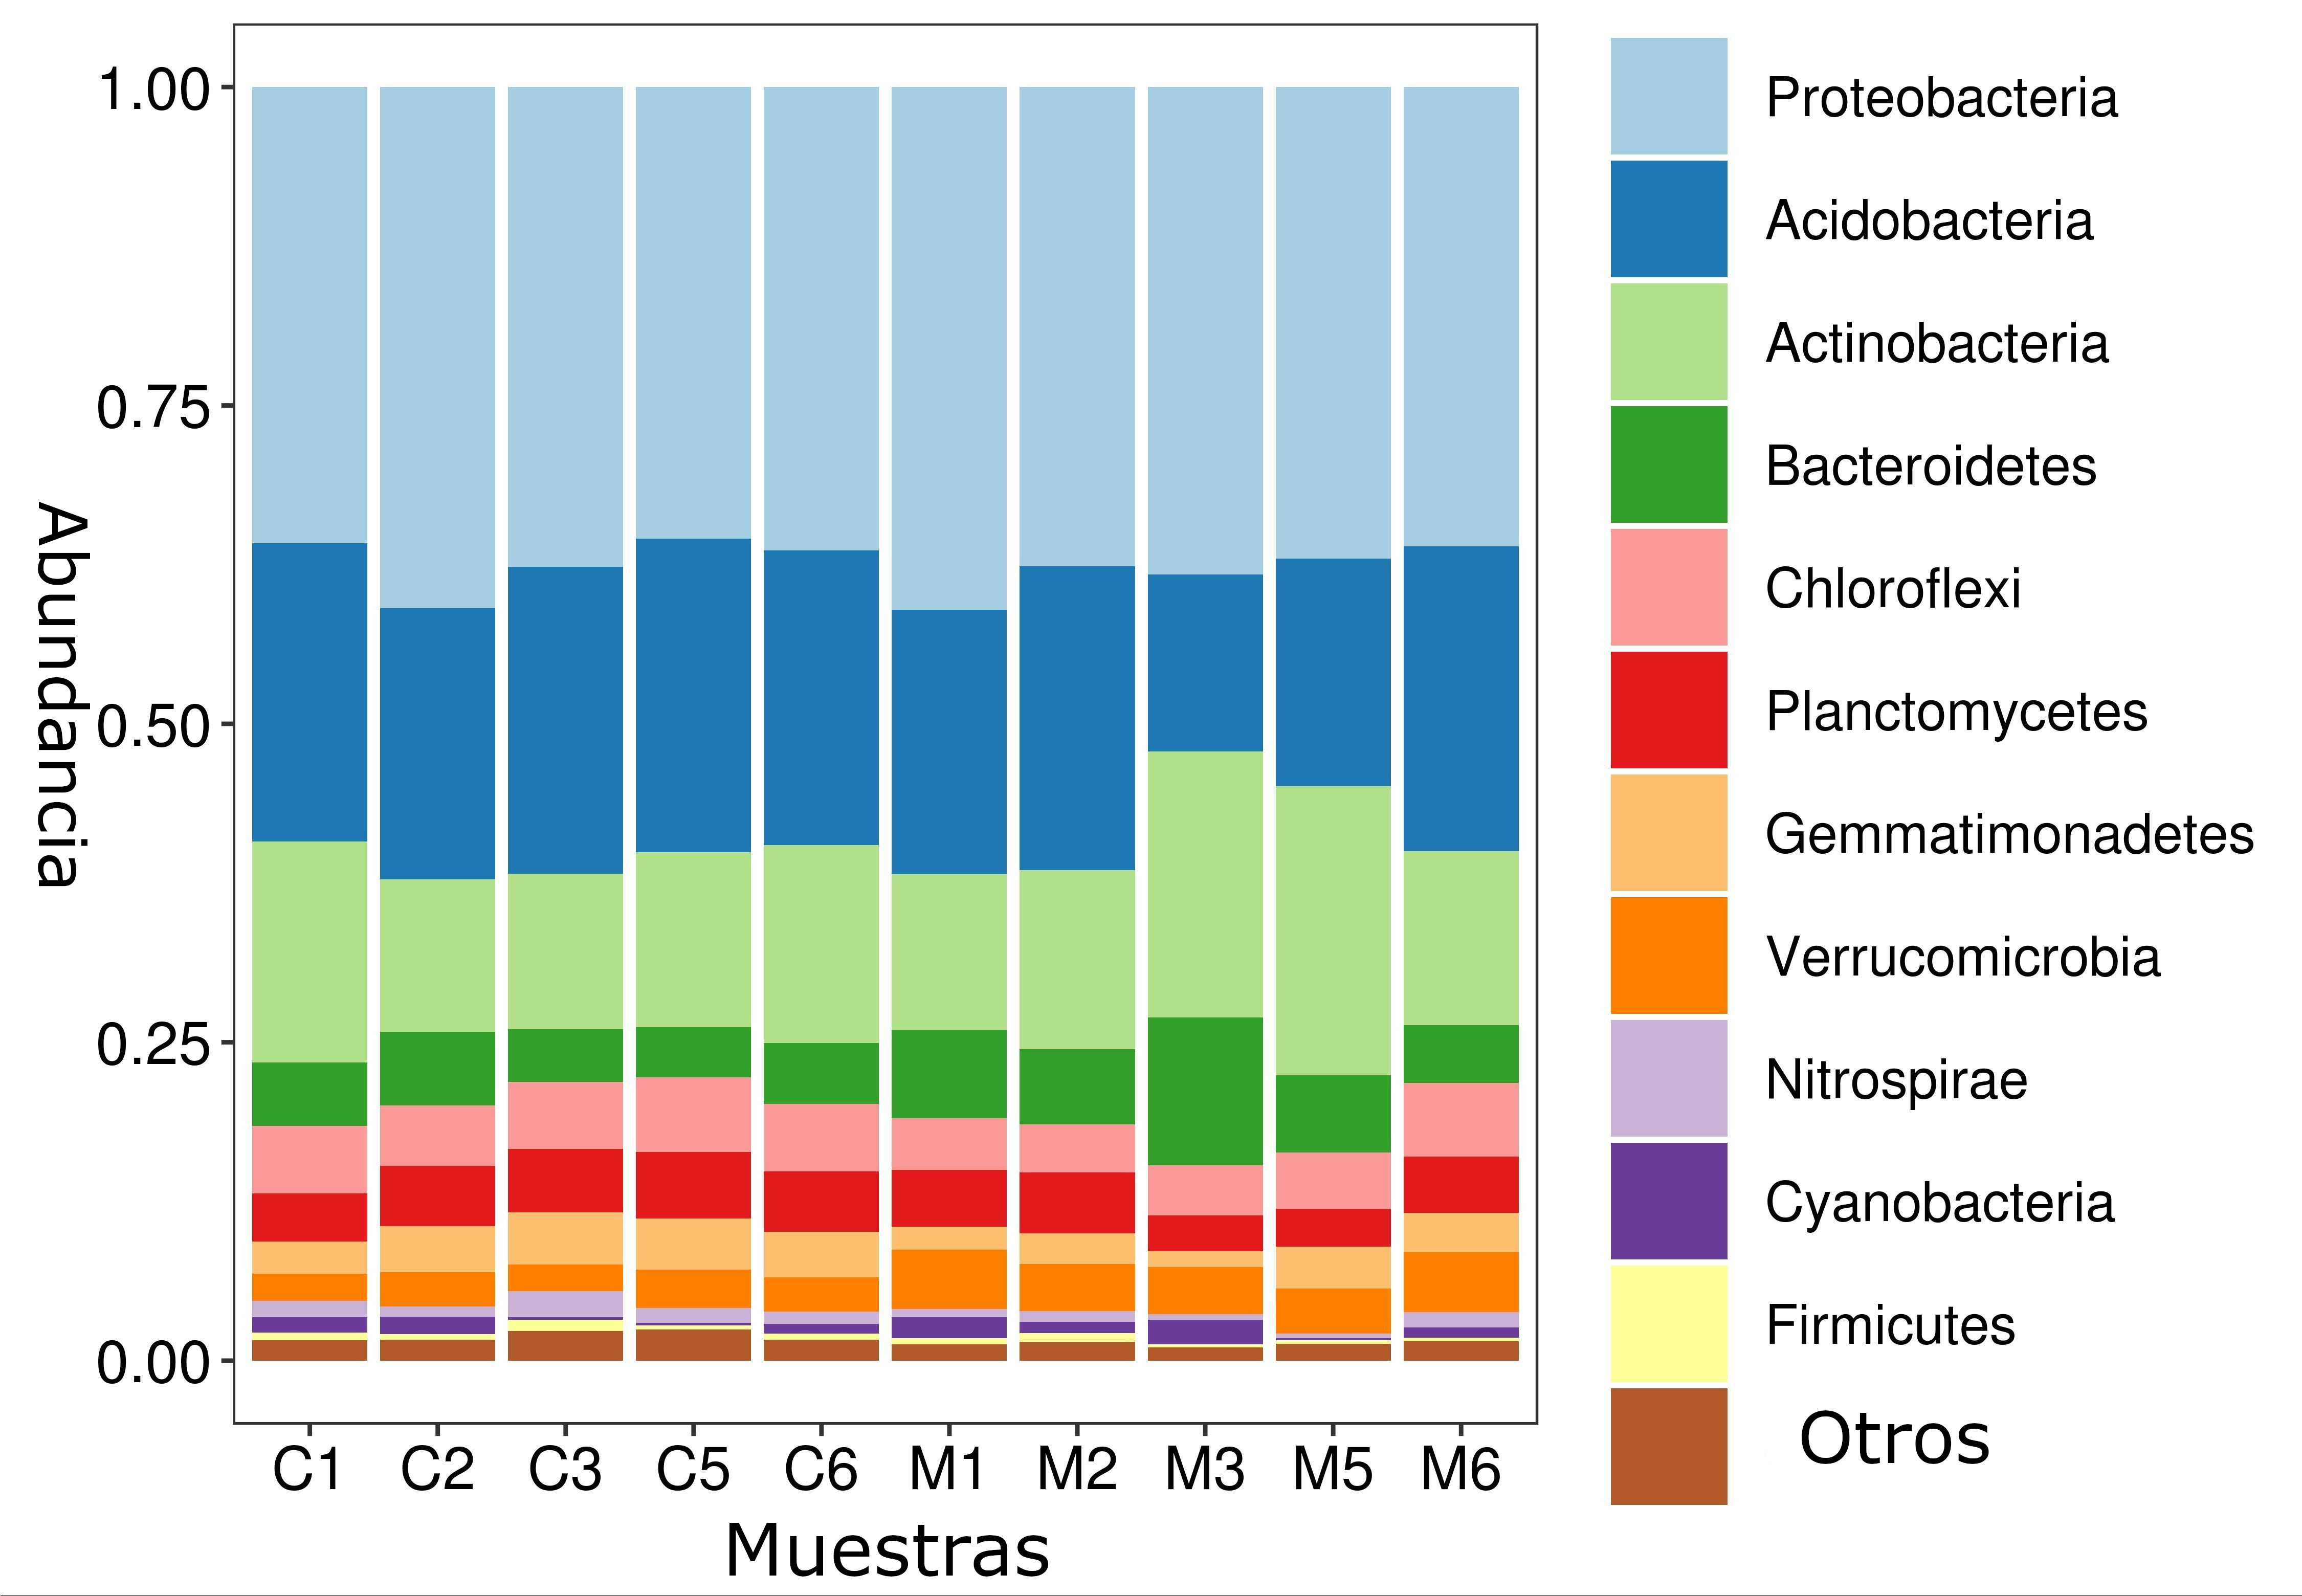
\includegraphics[width=16cm]{figuras/IMG_10}
\caption*{\textbf{Figura 9.-} Abundancia relativa del filo de bacterias en suelos de la milpa de El Boxo de Cardonal estado de Hidalgo. Donde la letra C es la muestra control y la letra M es la muestra de suelo cerca de las raíces de maiz.}
\label{Figura 10}
\end{figure}
\section{Importancia de \textit{Actinobacteria}}
El filo \textit{Actinobacteria} está constituido por bacterias Gram positivas \autocite{Kirchman2012}, y algunos géneros que lo comprenden, forman una relación de beneficio con las plantas. Dentro de las funciones que desempeñan son: ciclado de nutrientes, fijación de nitrógeno, solubilización de minerales y síntesis de antibióticos. Este último es de gran utilidad ya que la planta se defiende de agentes patógenos \autocite{Barka2015}.
\par
Dicho lo anterior, mediante la determinación de los géneros que componen \textit{Actinobacteria} en el suelo de las milpas, se plantean estrategias para su aislamiento y cultivo. Una vez cultivados, se pueden realizar pruebas de presencia de antibióticos u otras actividades, por ejemplo, para su empleo como agentes de control biológico. En este sentido, \textcite{van-der-Heul2018} menciona que distintas empresas biotecnológicas han cultivado algunas cepas de \textit{Actinobacteria} que consideran como “raras” (llamadas así por lo poco estudiadas) dada su importancia en el descubrimiento de nuevos productos naturales. Sin embargo, este estudio hace hincapié en que diversas cepas son difíciles de cultivar, por lo que es necesario desarrollar nuevas herramientas genéticas que caractericen las cepas de manera más eficiente. Una cepa de \textit{Actinobacteria} aislada de suelos de El Boxo, mostró actividad antifúngica sobre \textit{Fuzarium graminearum}en pruebas de laboratorio, por lo que estos microorganismos podrían jugar un papel en la protección de las plantas ante enfermedades en estos suelos (Cabrera-Ruiz et al., manuscrito en preparación). 
\section{Abundancia de \textit{Verrucomicrobia}}
Se encontró que el filo \textit{Verrucomicrobia} presenta mayor abundancia en el suelo de raíz en comparación con el suelo libre de raíces. \textcite{Lopes2016} afirma que la rizosfera selecciona bacterias específicas, las cuales se encuentran en el suelo libre de raíces, ocasionando que la cantidad de bacterias aumente. Con base en eso, se puede decir que las raíces de maíz, en la milpa tradicional, seleccionan y aumentan la cantidad de bacterias del filo \textit{Verrucomicrobia}. \textcite{Navarrete2015} explica que este filo se relaciona principalmente con la fertilidad del suelo. Así, si existe una deficiencia o un alto nivel de \ce{P, N, K} la estructura de la comunidad y la abundancia de \textit{Verrucomicrobia} se verá afectada. Además, la abundancia de este grupo está directamente relacionada con la humedad y la profundidad del suelo \autocite{Buckley2001}.
\newpage
\section{Predicción de rutas metabólicas}
Las tablas de OTU’s obtenidas de QIIME 2 se ingresaron en PICRUSt; obteniendo los genes predichos para el suelo de las milpas de El Boxo. Posteriormente se compararon las abundancias de estos genes en las muestras asociadas a las raíces y de los controles de suelo. Los genes que resultaron significativamente diferentes (Wilcoxon, p \textless  0.05) fueron ingresados en KEGG Mapper, donde se observan las rutas metabólicas obtenidas. En general se encontraron diferencias significativas en las rutas que intervienen en: el metabolismo del carbono, la degradación de compuestos aromáticos, el metabolismo de aminoácidos, el metabolismo de amino azúcares, transportadores ABC y la biosíntesis de metabolitos secundarios. 
\subsection{Metabolismo del carbono}
El carbono es la fuente de energía principal para la vida. Las bacterias del suelo utilizan diversas rutas para metabolizar este compuesto, como la glucólisis (Fig. 10) o la ruta de las pentosas fosfato. En principio, para que las comunidades bacterianas accedan al carbono, se debe llevar a cabo un proceso de fijación (Anexo A), en donde se toma el \ce{CO2} de la atmósfera, para que los microorganismos y las plantas lo sinteticen en materia orgánica (azúcares, almidones, etc.), mediante la fotosíntesis. Posteriormente esta materia orgánica se distribuye en toda la comunidad a través de la cadena trófica, donde se metaboliza y almacena, para finalmente ser liberado devuelta a la atmósfera \autocite{Gougoulias2014}.
\begin{figure}[!h]
\addcontentsline{lof}{section}{\textbf{Figura 10.-} Ruta metabólica de glucólisis y gluconeogénesis.}
\centering
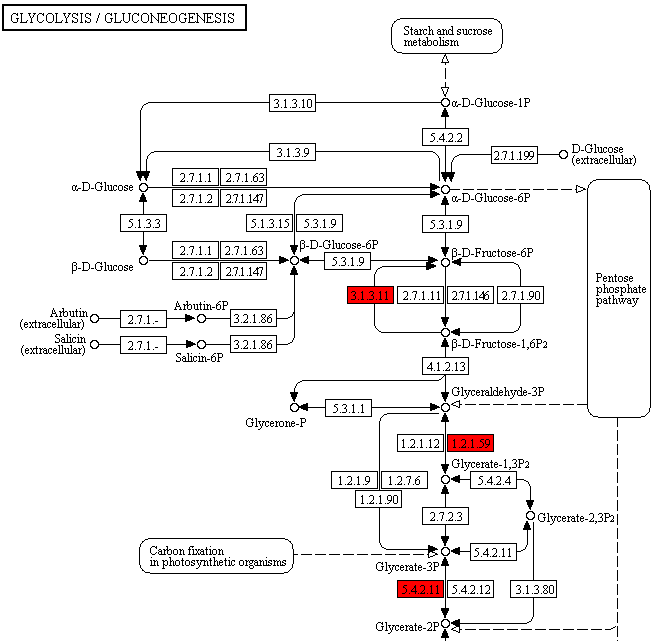
\includegraphics[width=15.59cm]{figuras/IMG_11}
\caption*{\textbf{Figura 10.-} Ruta metabólica obtenida de KEGG Mapper donde se observa el proceso de glucólisis y gluconeogénesis. Los genes marcados con rojo presentaron una mayor abundancia predicha en los suelos cercanos a las raíces de maíz en comparación con los controles (Anexo B).}
\label{Figura 11}
\end{figure}
\par
\textcite{Lange2015}, menciona que una mayor diversidad de vegetación en el suelo aumenta la entrada de carbono a la rizosfera. En consecuencia, se da una mayor actividad metabólica y un mejor almacenamiento del carbono. En el caso de la zona de estudio, ésta se caracterizó no solo por poseer plantas de maíz, sino que también de jitomate, frijol y calabaza, incluso algunos árboles frutales de peras, ciruelas y tejocotes, los cuales se encontraban alrededor de la milpa, de igual manera se encontraron diversas plantas silvestres que también son comestibles. Como resultado, se deduce que la milpa estudiada probablemente presenta un mejor intercambio de \ce{CO2} entre la atmósfera y el suelo, gracias a la gran diversidad vegetal y de comunidades bacterianas presentes. De igual manera, \textcite{Malik2018} argumentan que una menor intensificación agrícola en suelos con pH casi neutro mantiene un mejor almacenamiento de carbono lo que contribuye a una mayor síntesis de biomasa.
\par
En las muestras de suelo asociadas a las raíces de las plantas de maíz, se predijo un enriquecimiento de genes relacionados con el metabolismo del carbono, incluyendo la glucólisis (Fig. 10). Esto sugiere que en la vecindad de las raíces hay una mayor actividad de degradación del carbono. Probablemente, el aporte de exudados orgánicos de las plantas de utiliza como fuente de carbono por parte de las bacterias que habitan en esta zona, por lo que se incrementan los genes necesarios para su degradación. 
\subsection{Degradación de compuestos aromáticos}
El análisis realizado con PICRUSt de igual manera identificó algunas rutas que contribuyen a la degradación de compuestos aromáticos enriquecidos en la vecindad de las raíces (Fig. 11), que pueden optar por dos caminos, la degradación aeróbica o la anaeróbica. En cualquiera de los casos es necesario que la bacteria en cuestión sea capaz de desestabilizar el anillo benceno \autocite{Diaz2013}. \textcite{Mrozik2010} plantean el uso de bioaumentación para remediar suelos que estén contaminados con compuestos aromáticos. Por lo tanto, las bacterias de las milpas que realizan esta actividad podrían ser utilizadas para su aplicación biotecnológica en la biorremediación.
\begin{figure}[!h]
\addcontentsline{lof}{section}{\textbf{Figura 11.-} Ruta metabólica de degradación de compuestos aromáticos.}
\centering
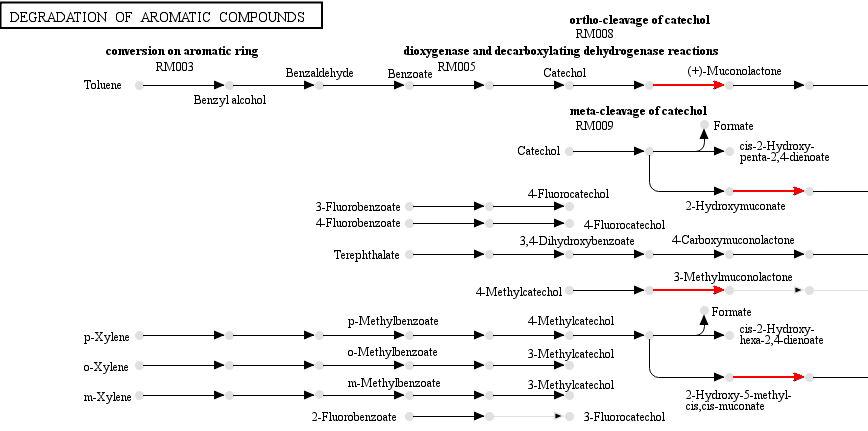
\includegraphics[width=14cm]{figuras/IMG_12}
\caption*{\textbf{Figura 11.-} Ruta metabólica de degradación de compuestos aromáticos (Anexo C).}
\label{Figura 12}
\end{figure}
\newpage
\subsection{Metabolismo de aminoácidos}
Las raíces de las plantas exudan diversos compuestos, tanto de alto como de bajo peso molecular. Dentro de los primeros se encuentran los aminoácidos, que son liberados al suelo donde pueden ser tomados por las raíces de otras plantas o por la microbiota que esté alrededor \autocite{Badri2009}. Las rutas metabólicas encontradas enriquecidas en el suelo de las raíces de plantas de maíz de la milpa de El Boxo comprenden el metabolismo de glicina, serina, treonina, arginina, prolina, tirosina y glutatión, así como biosíntesis de lisina (Fig. 12).
\par
\textcite{Moe2013} menciona que el papel de los aminoácidos en la rizosfera es el de: fungir como intermediaros en el metabolismo, servir como estructura en productos naturales, actuar como cofactores en reacciones enzimáticas y ser reguladores de la fisiología de las células; de igual manera menciona que sirven como fuente de nitrógeno y carbono.
\par
De las rutas de aminoácidos determinadas, la glicina y arginina funcionan como fuentes de carbono para los microorganismos \autocite{Pizer1965}. \textcite{Haney2018} determinaron el consumo de arginina, glicina y otros aminoácidos por parte de las bacterias en la rizosfera, cuantificando este consumo mediante la liberación de \ce{CO2}. Afirman que una buena cantidad presente de estos compuestos en la rizosfera es beneficioso para los microorganismos y para los cultivos.
\par
Aún más, existe otro papel importante de algunos aminoácidos, que es el de actuar como herbicidas. Donde inhiben el crecimiento de plantas, aunque esto depende del tipo de planta y del tipo de aminoácido que se utiliza \autocite{Fernandez-Aparicio2017}. Esto es de gran importancia puesto que, si en el futuro se desarrollan bioherbicidas de mayor rendimiento, entonces se podrían prescindir de los productos químicos que dañan los cultivos y el suelo.
\par
Los aminoácidos son los compuestos con los que se sintetizan las proteínas \autocite{Ambrogelly2006}. En las muestras de suelos asociados a las raíces se predijo una mayor abundancia de genes involucrados en la síntesis de aminoácidos que en los suelos alejados de las plantas. Estos resultados sugieren que, en cercanía con las raíces, las comunidades microbianas presentan un metabolismo más activo, con mayor necesidad de síntesis de proteínas.
\begin{figure}[!h]
\addcontentsline{lof}{section}{\textbf{Figura 12.-} Ruta metabólica donde se observa el proceso de la biosíntesis de aminoácidos.}
\centering
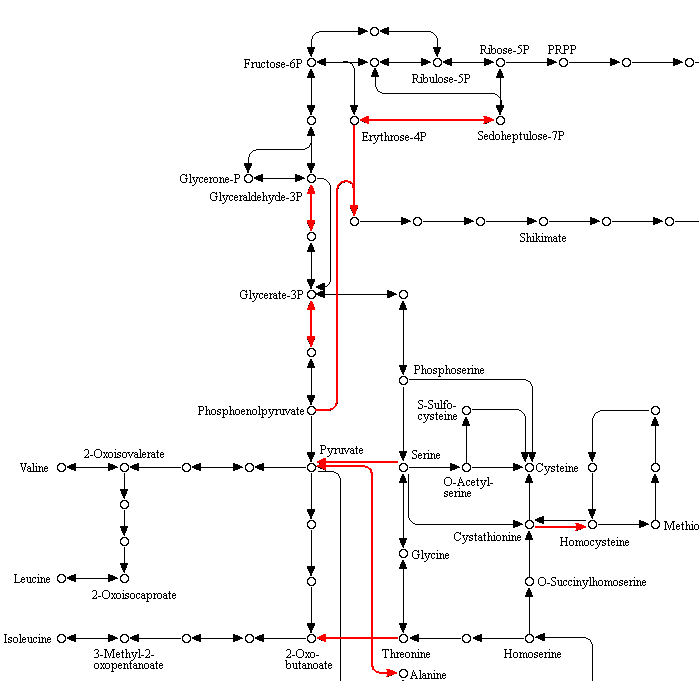
\includegraphics[width=15.59cm]{figuras/IMG_13}
\caption*{\textbf{Figura 12.-} Ruta metabólica donde se observa el proceso de la biosíntesis de aminoácidos. Donde las flechas rojas indican las reacciones químicas que llevan a cabo las bacterias de El Boxo (Anexo D).}
\label{Figura 13}
\end{figure}
\newpage
\subsection{Metabolismo de amino azúcares}
En la predicción de las rutas metabólicas, también se encontró una mayor abundancia de genes para el metabolismo de amino azúcares (Fig. 13), los cuales constituyen las paredes celulares de las bacterias, además de que intervienen en el ciclo del nitrógeno. \textcite{Roberts2007} hallaron en sus pruebas de mineralización de \ce{CO2} que la concentración de amino azúcares (glucosamina) era menor a la que esperaban. Su hipótesis fue que esto se debía a que existe una rápida remoción de glucosamina en lugar de una baja tasa de producción. Concluyen que existe un alto reciclaje de este compuesto lo que quiere decir que figura como un buen sustrato para el metabolismo microbiano. Nuevamente, estos resultados sugieren un metabolismo más activo en la vecindad de las raíces, posiblemente por un incremento en la disponibilidad de carbono orgánico, derivado de las plantas.
\begin{figure}[!ht]
\addcontentsline{lof}{section}{\textbf{Figura 13.-} Ruta metabólica del metabolismo de amino azúcares.}
\centering
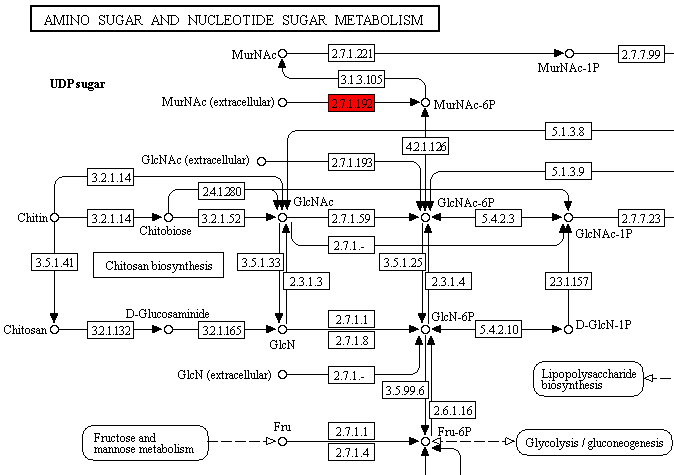
\includegraphics[width=15.59cm]{figuras/IMG_14}
\caption*{\textbf{Figura 13.-} Ruta donde se observa el metabolismo de amino azúcares. El gen marcado de rojo presentó mayor abundancia predicha en el suelo cercano a las raíces de maíz (Anexo E).}
\label{Figura 14}
\end{figure}
\newpage
\subsection{Transportadores ABC}
Los transportadores ABC llevan moléculas a través de las membranas de las células, mediante un gasto energético. Varios de ellos se encontraron enriquecidos en las muestras colectadas en las raíces del maíz (Fig. 14). En bacterias, fungen como transportadores de metabolitos primarios, lípidos, antibióticos y proteínas, entre muchos otros compuestos \autocite{Kang2011}.
\par
Los que se encontraron enriquecidos, transportan azúcares, oligosacáridos y aminoácidos, así como nutrientes como el manganeso y el sulfato. El enriquecimiento de estos genes cerca de las raíces sugiere la utilización de moléculas orgánicas derivadas de las plantas en estas bacterias, las cuales necesitan incorporarse para su metabolismo. Asimismo, algunas de las moléculas transportadas por este mecanismo podrían constituir señales químicas, tanto de las plantas a las bacterias, como de las bacterias a las plantas. Esto se podría verificar experimentalmente en trabajos futuros.
\begin{figure}[!h]
\addcontentsline{lof}{section}{\textbf{Figura 14.-} Transportadores ABC predichos por PICRUSt.}
\centering
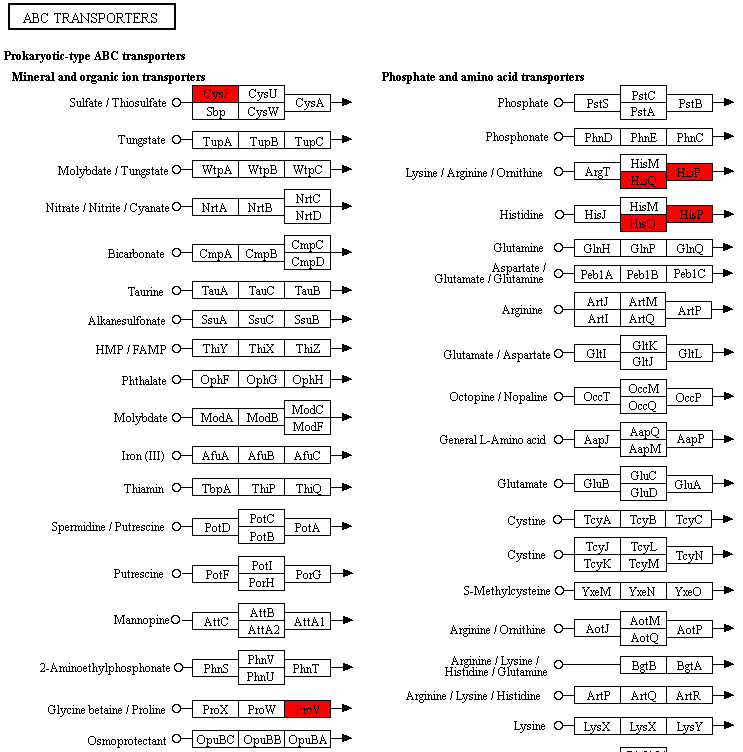
\includegraphics[width=10cm]{figuras/IMG_15}
\caption*{\textbf{Figura 14.-} Algunos de los transportadores ABC predichos por PICRUSt. Los genes marcados con rojo presentaron una mayor abundancia predicha en los suelos cercanos a las raíces de maíz en comparación con los controles (Anexo F).}
\label{Figura 15}
\end{figure}
\newpage
\subsection{Biosíntesis de metabolitos secundarios}
Los metabolitos secundarios son esenciales en las interacciones biológicas, y podrían estar involucrados, directa o indirectamente, en las que se llevan a cabo entre planta-bacteria. Se encontraron diversos genes que intervienen en la síntesis de metabolitos secundarios enriquecidos en los suelos adyacentes a las raíces del maíz. Uno de los grupos más activos en la producción de estos compuestos en el suelo son las \textit{Actinobacterias} \autocite{Barka2015}. Como se ha mencionado antes, \textit{Actinobacteria} es un filo abundante en el suelo de milpas, en el que se encuentran diversos tipos de bacterias. De éstas, la familia \textit{Streptomycetaceae} es conocida por su capacidad biosíntesis de diversos compuestos de gran importancia, tales como antibióticos y otros metabolitos secundarios, como insecticidas y herbicidas \autocite{Barka2015}. La cantidad de metabolitos secundarios se regula por la disponibilidad de nitrógeno, carbono y fosfato. La tabla 5 muestra algunos de los tipos de antibióticos y metabolitos secundarios que fueron predichos por PICRUSt, con mayor abundancia en las muestras de las raíces.
%\begin{table}[!h]
\addcontentsline{lot}{section}{\textbf{Tabla 6.-} Relación de los metabolitos secundarios predichos por PICRUSt.}
%\centering
\begin{longtable}[c]{ccm{5cm}}
%\begin{tabularx}{\linewidth}{*{3}{>{\hangindent=1em\hangafter=1\Centering}X}}
%\addcontentsline{lot}{section}{\textbf{Tabla 6.-} Se muestra la bacteria productora, el compuesto y el tipo de función.}
\caption*{\textbf{Tabla 6.-} Relación de los metabolitos secundarios predichos por PICRUSt con mayor abundancia predicha en los suelos cercanos a las raíces de maíz en comparación con los controles con la bacteria productora y su función.} \label{Tabla 6}\\
\toprule[0.5mm]
Agente bioactivo & Agentes productores & Función  \\ 
\midrule
\multirow{3}{*}{Cefamicina C} & \textit{Streptomyces cattleya} & \\
& \textit{Streptomyces clavuligerus} & Agente Antimicrobiano\\
& \textit{Armycolaptosis albispora} & \\ 
\hline
\multirow{5}{*}{Carbapenem} & \textit{Serratia sp.} & \\
& \textit{Dickeya chrysantemi} & \\
& \textit{Pantoea sp.} & Agente antibacteriano\\ 
& \textit{Photorhabdus laoumondii} & \\ 
& \textit{Providencia rettgeri} & \\ 
\hline
Nocardicina A & \textit{Actinosynnema mirum} & Agente antimicrobiano  \\ 
\hline
Validamicina A & \textit{Streptomyces hygroscopicus} & Agroquimico antifúngico  \\ 
 \hline
\multirow{3}{*}{Pirrolnitrina} & \textit{Serratia sp.} & \\
& \textit{Pseudomona sp.} & Medicamento antimicótico\\
& \textit{Burkholderia sp.} &\\ 
\hline
\multirow{2}{*}{Estaurosporina} & \textit{Streptomyces rubrolavendulae} & Metabolito secundario \\
& \textit{Streptomyces clavuligerus} & \\
\hline
\multirow{3}{*}{Violaceina} & \textit{Chromobacterium violaceum} & Agente antibacteriano\\
& \textit{Janthinobacterium agaricidamnosum} & Agente antifúngico\\

& \textit{Massilia sp.} & Inductor de apoptosis\\
\hline
Piocianina & \textit{Pseudomonas aeruginosa} & Agente antibacteriano, Pigmento biológico

Factor de virulencia \\
\hline
\multirow{3}{*}{Prodigiosina} & \textit{Serratia sp.} & Agente Antimicrobiano\\
& \textit{Vibrio gazogenes} & Pigmento biológico \\
& \textit{Pseudoalteromonas rubra} & Inductor de apoptosis\\
\hline
\multirow{2}{*}{Undecilprodigiosina} & \textit{Streptoymces coelicolor} & Pigmento biológico\\
& \textit{Streptomyces levidans} & Medicamento \\
\hline
Bacilisina & \textit{Bacillus subtilis} & Agente antibacteriano

Agente antifúngico \\
\hline
\multirow{2}{*}{Pentalenolactona} & \textit{Streptomyces bingchengensis} & Agente antibacteriano \\
& \textit{Streptomyces cyaneogriseus} & Agente antifúngico \\
\bottomrule[0.5mm]
%\end{tabularx}
\end{longtable}
%\end{table}
\par
La mayoría de estos compuestos son antimicrobianos y antifúngicos, lo que indica que un estudio más profundo sobre alguno de estos agentes puede ser de gran utilidad para en el futuro desarrollar un mejor biocontrol sobre las plagas existentes, además que sean amigables con los cultivos y con el suelo.
\par
\textcite{Barka2015} reporta el papel que tiene \textit{Actinobacteria} como productor de agentes antimicrobianos y antibióticos, así como en el mejoramiento del crecimiento de plantas y resistencia a enfermedades. De igual manera argumenta que este filo es de gran importancia por su función como reciclador de biomateriales y como control biológico de plagas.
En otro estudio, se aislaron \textit{Actinobacterias} de la misma milpa de El Boxo, y uno de estos aislados presentó actividad antifúngica contra un hongo fitopatógeno (Cabrera-Ruiz, comunicación personal). Esto es consistente con los resultados obtenidos con PICRUSt en esta tesis, y sugiere que este grupo de microorganismos podría estar involucrado en la protección de las plantas ante posibles enfermedades fúngicas.
\chapter{Conclusiones y Prospectivas}
\section{Conlusiones}
\begin{itemize}
\item Las plantas de maíz tienen una gran influencia sobre las comunidades microbianas que habitan en la vecindad de sus raíces y viceversa.
\item Entre las rutas metabólicas que se hallaron en las comunidades microbianas de las raíces, se encuentran algunas relacionadas con el metabolismo del carbono y la degradación de diferentes compuestos orgánicos, como aminoácidos y compuestos aromáticos, lo que sugiere que estas comunidades son activas en la degradación de compuestos orgánicos provenientes de las plantas.
\item Un patrón observado en las comunidades microbianas enriquecidas en la vecindad de las raíces de las plantas de maíz, fue la presencia de genes posiblemente relacionados con interacciones biológicas, como genes para la síntesis de metabolitos secundarios. Esto sugiere que existen interacciones directas o indirectas, entre las plantas y algunas bacterias enriquecidas en las raíces. 
\item Algunas de las rutas metabólicas en los suelos de las raíces del maíz podrían aprovecharse con fines biotecnológicos, como la síntesis de metabolitos secundarios y la degradación de compuestos aromáticos.
\end{itemize}
\newpage
\section{Prospectivas}
\begin{itemize}
\item Lograr una determinación precisa de los genomas completos de éste agroecosistema, mediante metagenómica de shotgun, para detectar una o mas cepas en concreto que posean los genes necesarios para llevar a cabo las rutas metabólicas mas prometedoras detectadas en este proyecto, por ejemplo aquellas relacionadas con la interacción planta-microorganismo.
\item Una vez detectadas estas cepas, se propone planear una estrategia para su aislamiento en el laboratorio, tomando en cuenta las rutas metabólicas presentes en sus genomas, en particular, si se detectan carencias en sus capacidades de sintetizar ciertos componentes componentes celulares esenciales. En caso de existir dichas carencias, se agregarían en el medio para hacer posible su aislamiento
\item Las cepas aisladas con esta estrategia se formularían como biofertilizantes para su aplicación en el campo, con el fin aumentar su abundancia y actividad.
\item Se propone tratar de mejorar o desarrollar un algoritmo mediante inteligencia artificial más eficiente que el utilizado por PICRUSt debido a su sesgo en la inferencia de genes de 16S.
\end{itemize}
\renewcommand{\appendixname}{Anexo}
%\renewcommand{\appendixpagename}{Anexo}
\appendix
\cleardoublepage
\addtocontents{toc}{\bigskip}
\addcontentsline{toc}{part}{Anexos}
\titleformat{\chapter}[display]
  {\normalfont\large\bfseries}% <- font for label "Appendix A", default \huge
  {\chaptertitlename\ \thechapter}
  {20pt}
  {\large}% <- font for title, default \Huge
\chapter{Ruta metabólica de la fijación del carbono}
\begin{figure}[!h]
\centering
\centerline{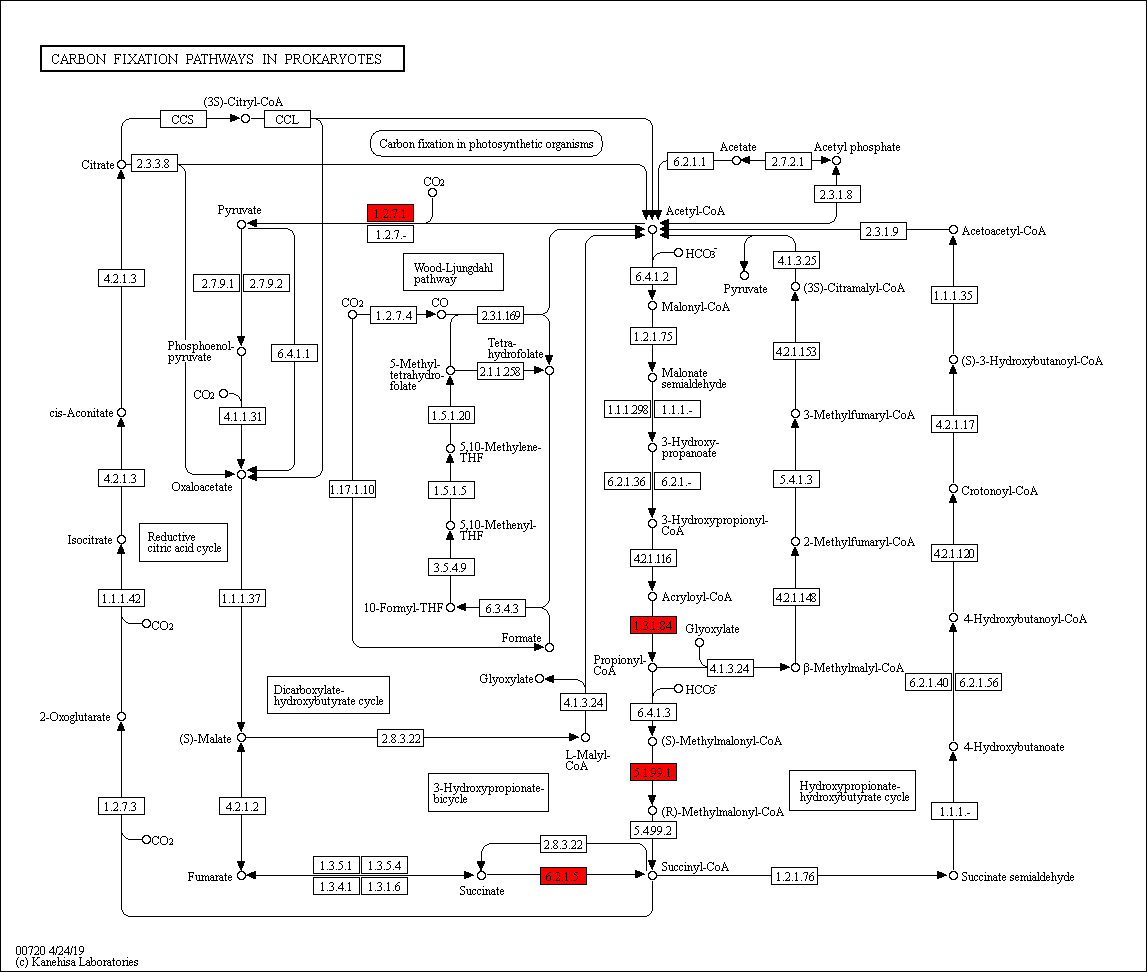
\includegraphics[width=18cm]{apendices/A-1}}
\caption*{\textbf{Anexo A.-} Ruta metabólica de fijación del carbono, los genes en rojo indican una mayor abundancia de genes predichos.}
\end{figure}
\chapter{Ruta metabólica de la glucólisis/gluconeogénesis}
\begin{figure}[!h]
\centering
\centerline{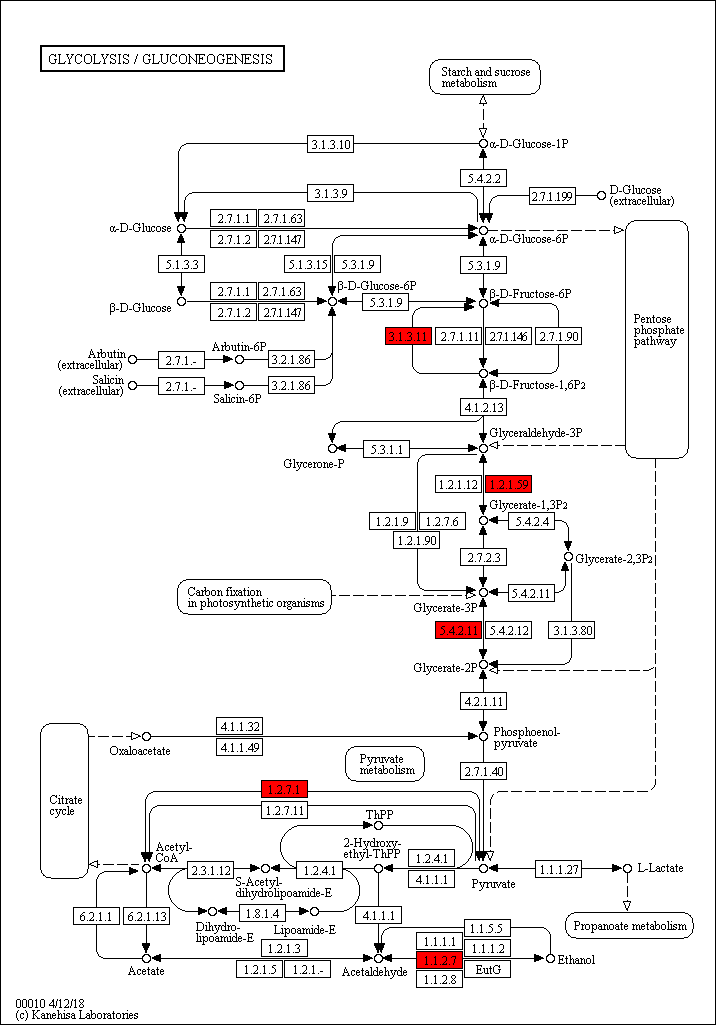
\includegraphics[scale=0.44]{apendices/B-2}}
\caption*{\textbf{Anexo B.-} Ruta metabólica que presenta la glucólisis/gluconeogénesis donde de color rojo se presentan los genes con mayor abundancia.}
\end{figure}
\chapter{Ruta metabólica de degradación de compuestos aromáticos}
\begin{figure}[!h]
\centerline{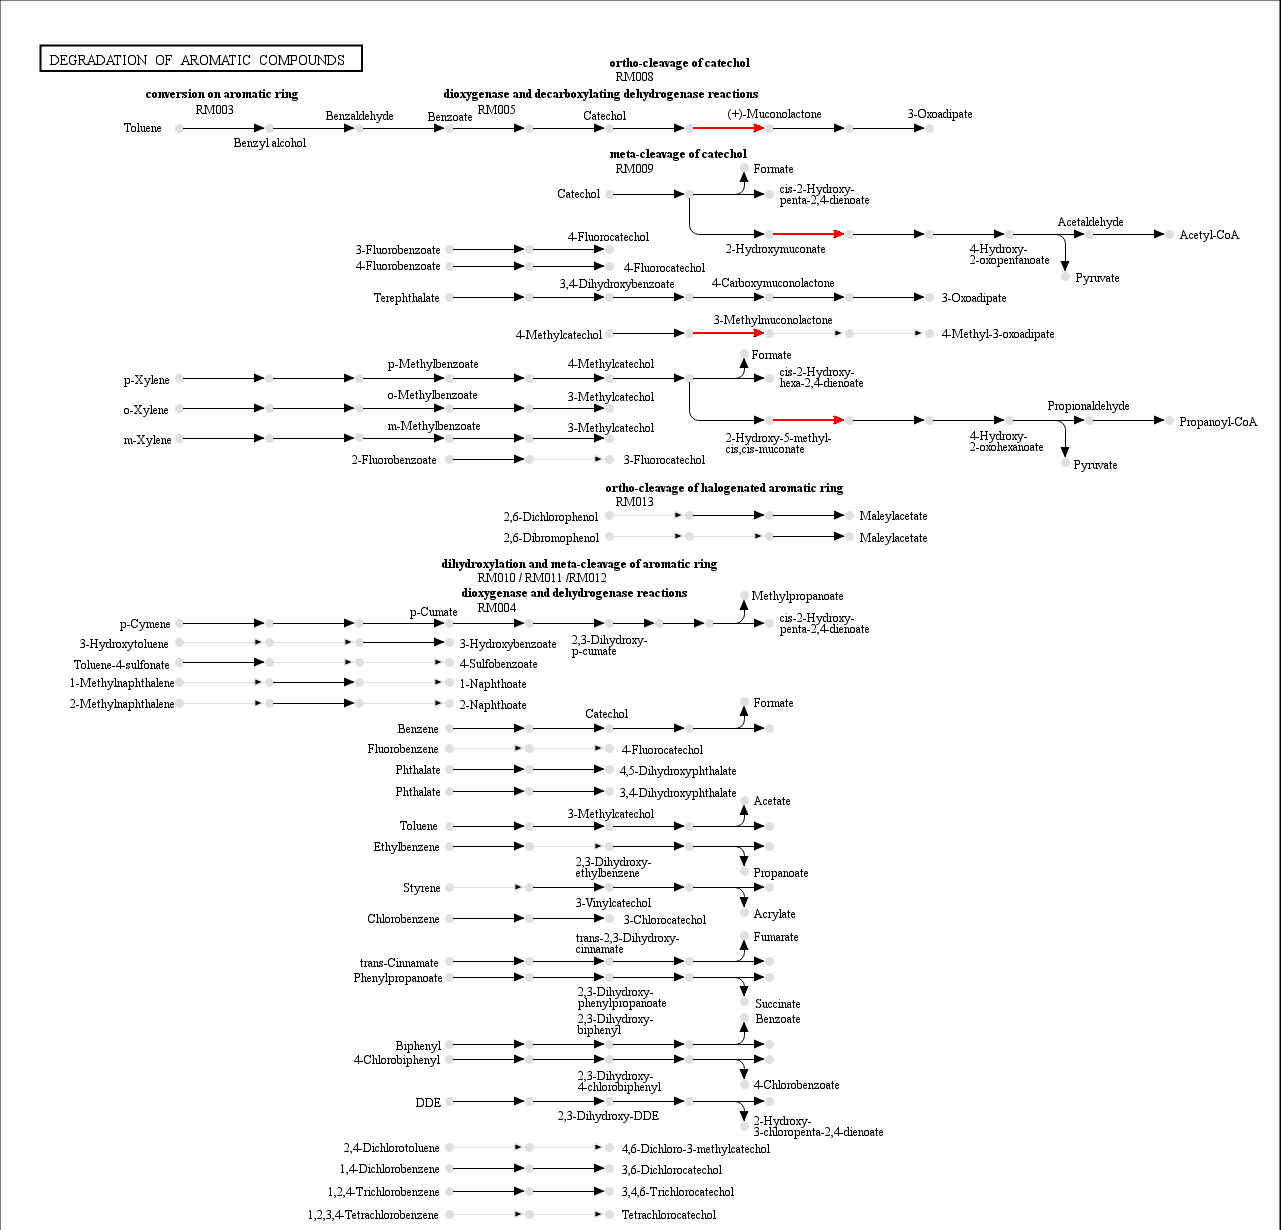
\includegraphics[width=\linewidth,height=\textheight,keepaspectratio]{apendices/C-3 A}}
\end{figure}
\begin{figure}
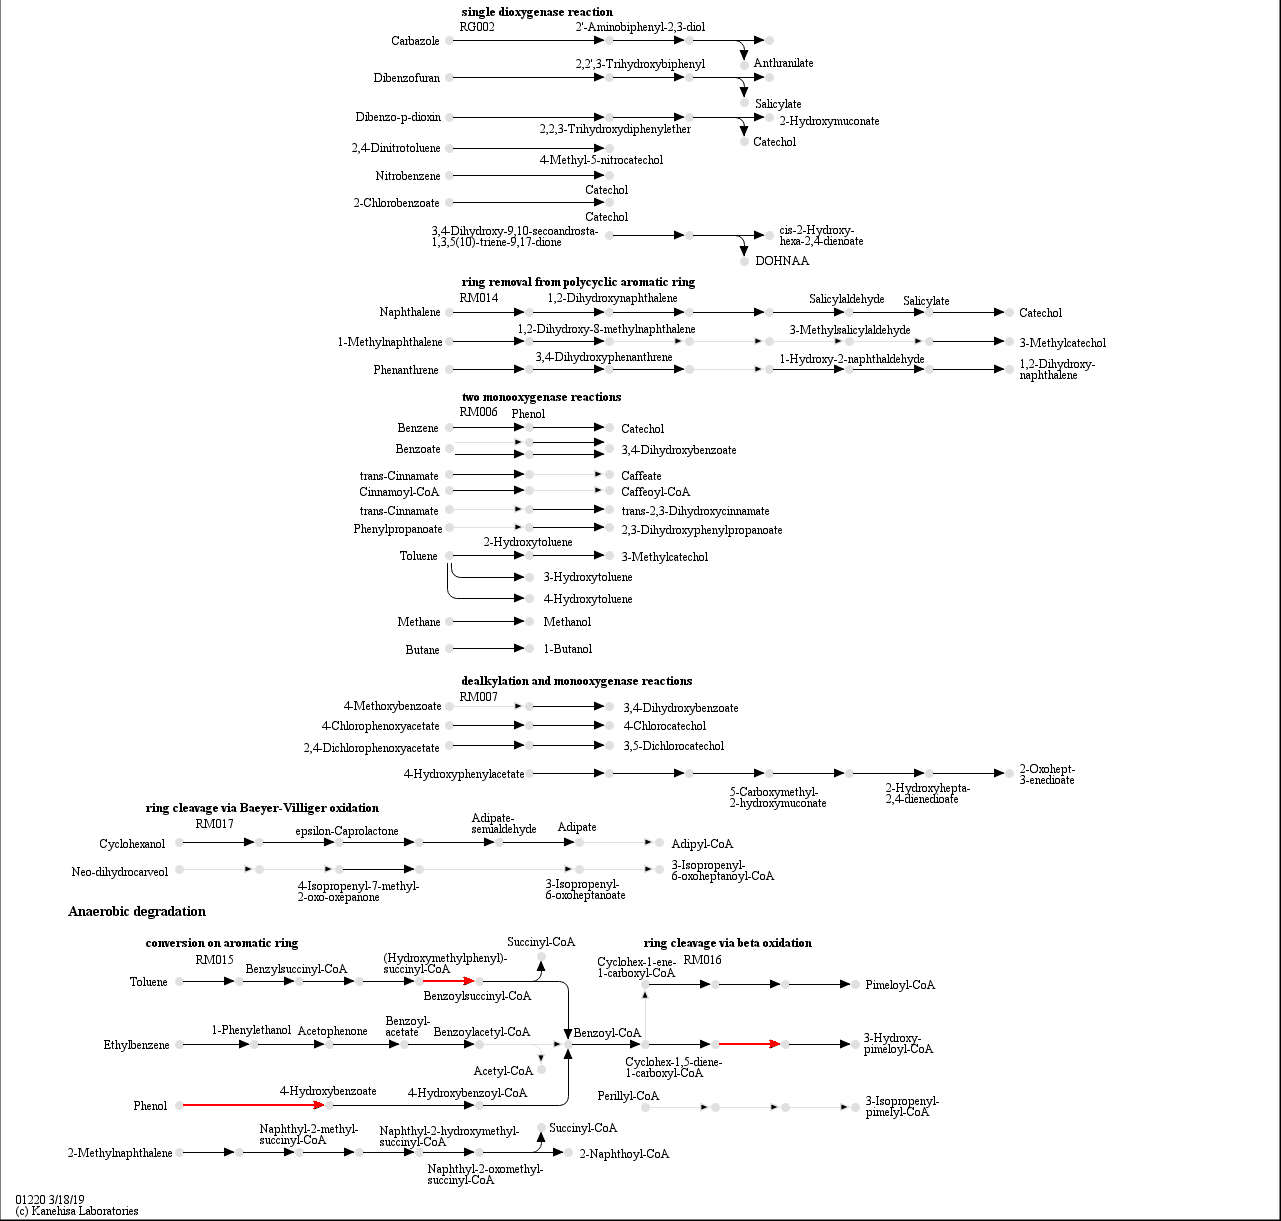
\includegraphics[width=\linewidth,height=\textheight,keepaspectratio]{apendices/C-3 B}
\caption*{\textbf{Anexo C.-} Ruta metabólica donde se observan de rojo los genes expresados para la degradación de compuestos aromáticos.}
\end{figure}
\chapter{Ruta metabólica de aminoácidos}
\begin{figure}[!h]
\centering
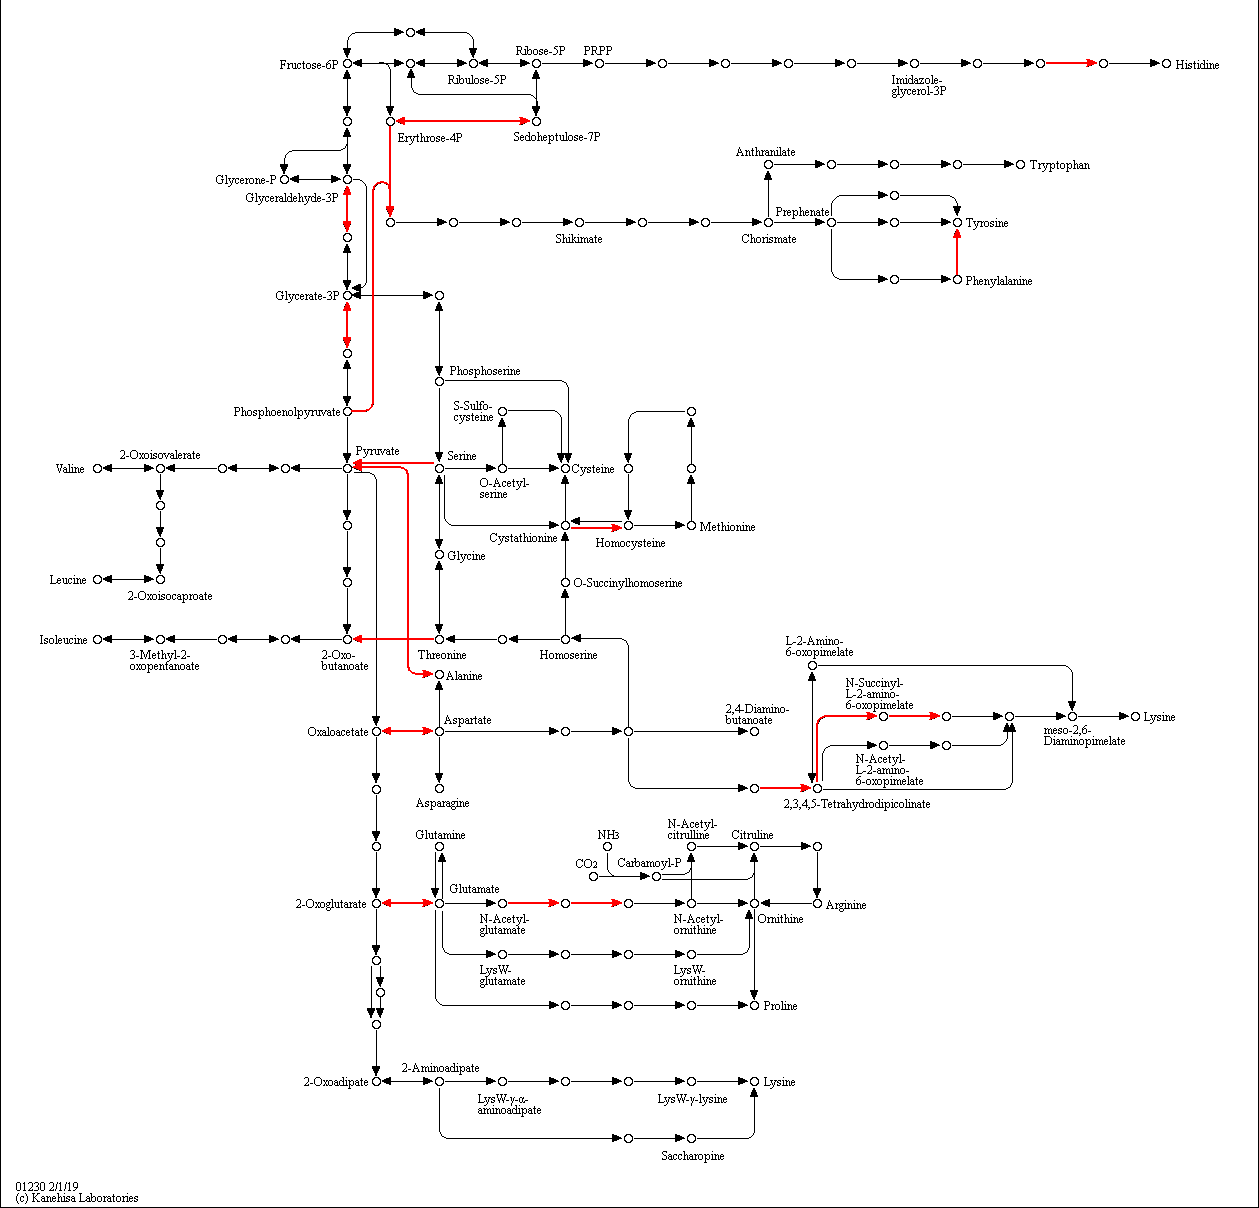
\includegraphics[scale=0.35]{apendices/D-4}
\caption*{\textbf{Anexo D.-} Ruta metabólica de aminoácidos, las flechas en rojo indican los genes expresados con mayor abundancia.}
\end{figure}
\chapter{Ruta metabólica de metabolismo de amino azúcares}
\begin{figure}[!h]
\centering
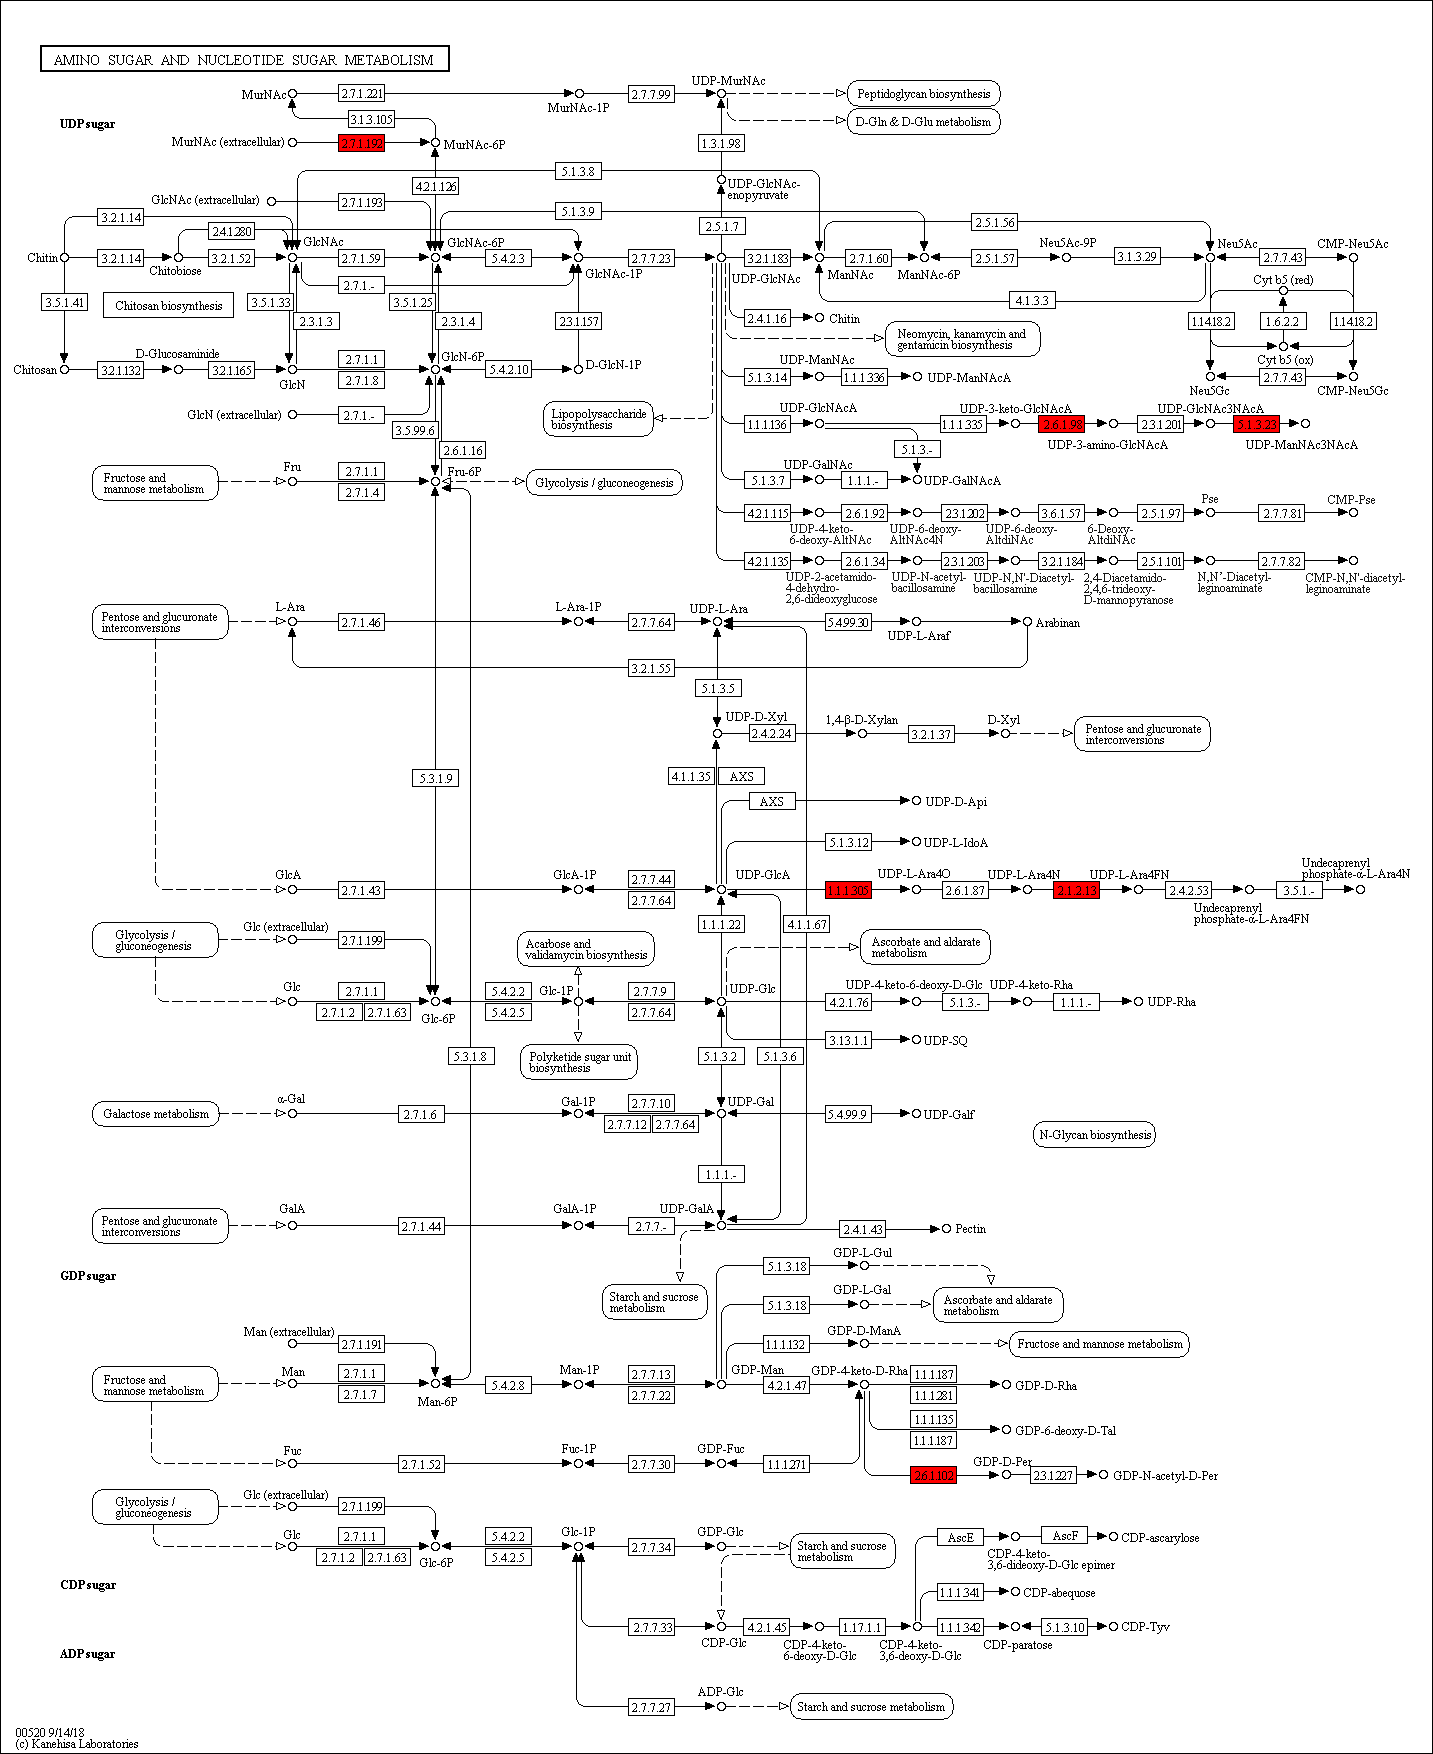
\includegraphics[scale=0.25]{apendices/E-5}
\caption*{\textbf{Anexo E.-} En esta ruta se muestra el metabolismo de aminoazúcares, de rojo se presentan los genes con mayor abundancia.}
\end{figure}
%\begin{landscape}
\chapter{Ruta de los transportadores ABC}
\begin{figure}[!h]
\centering
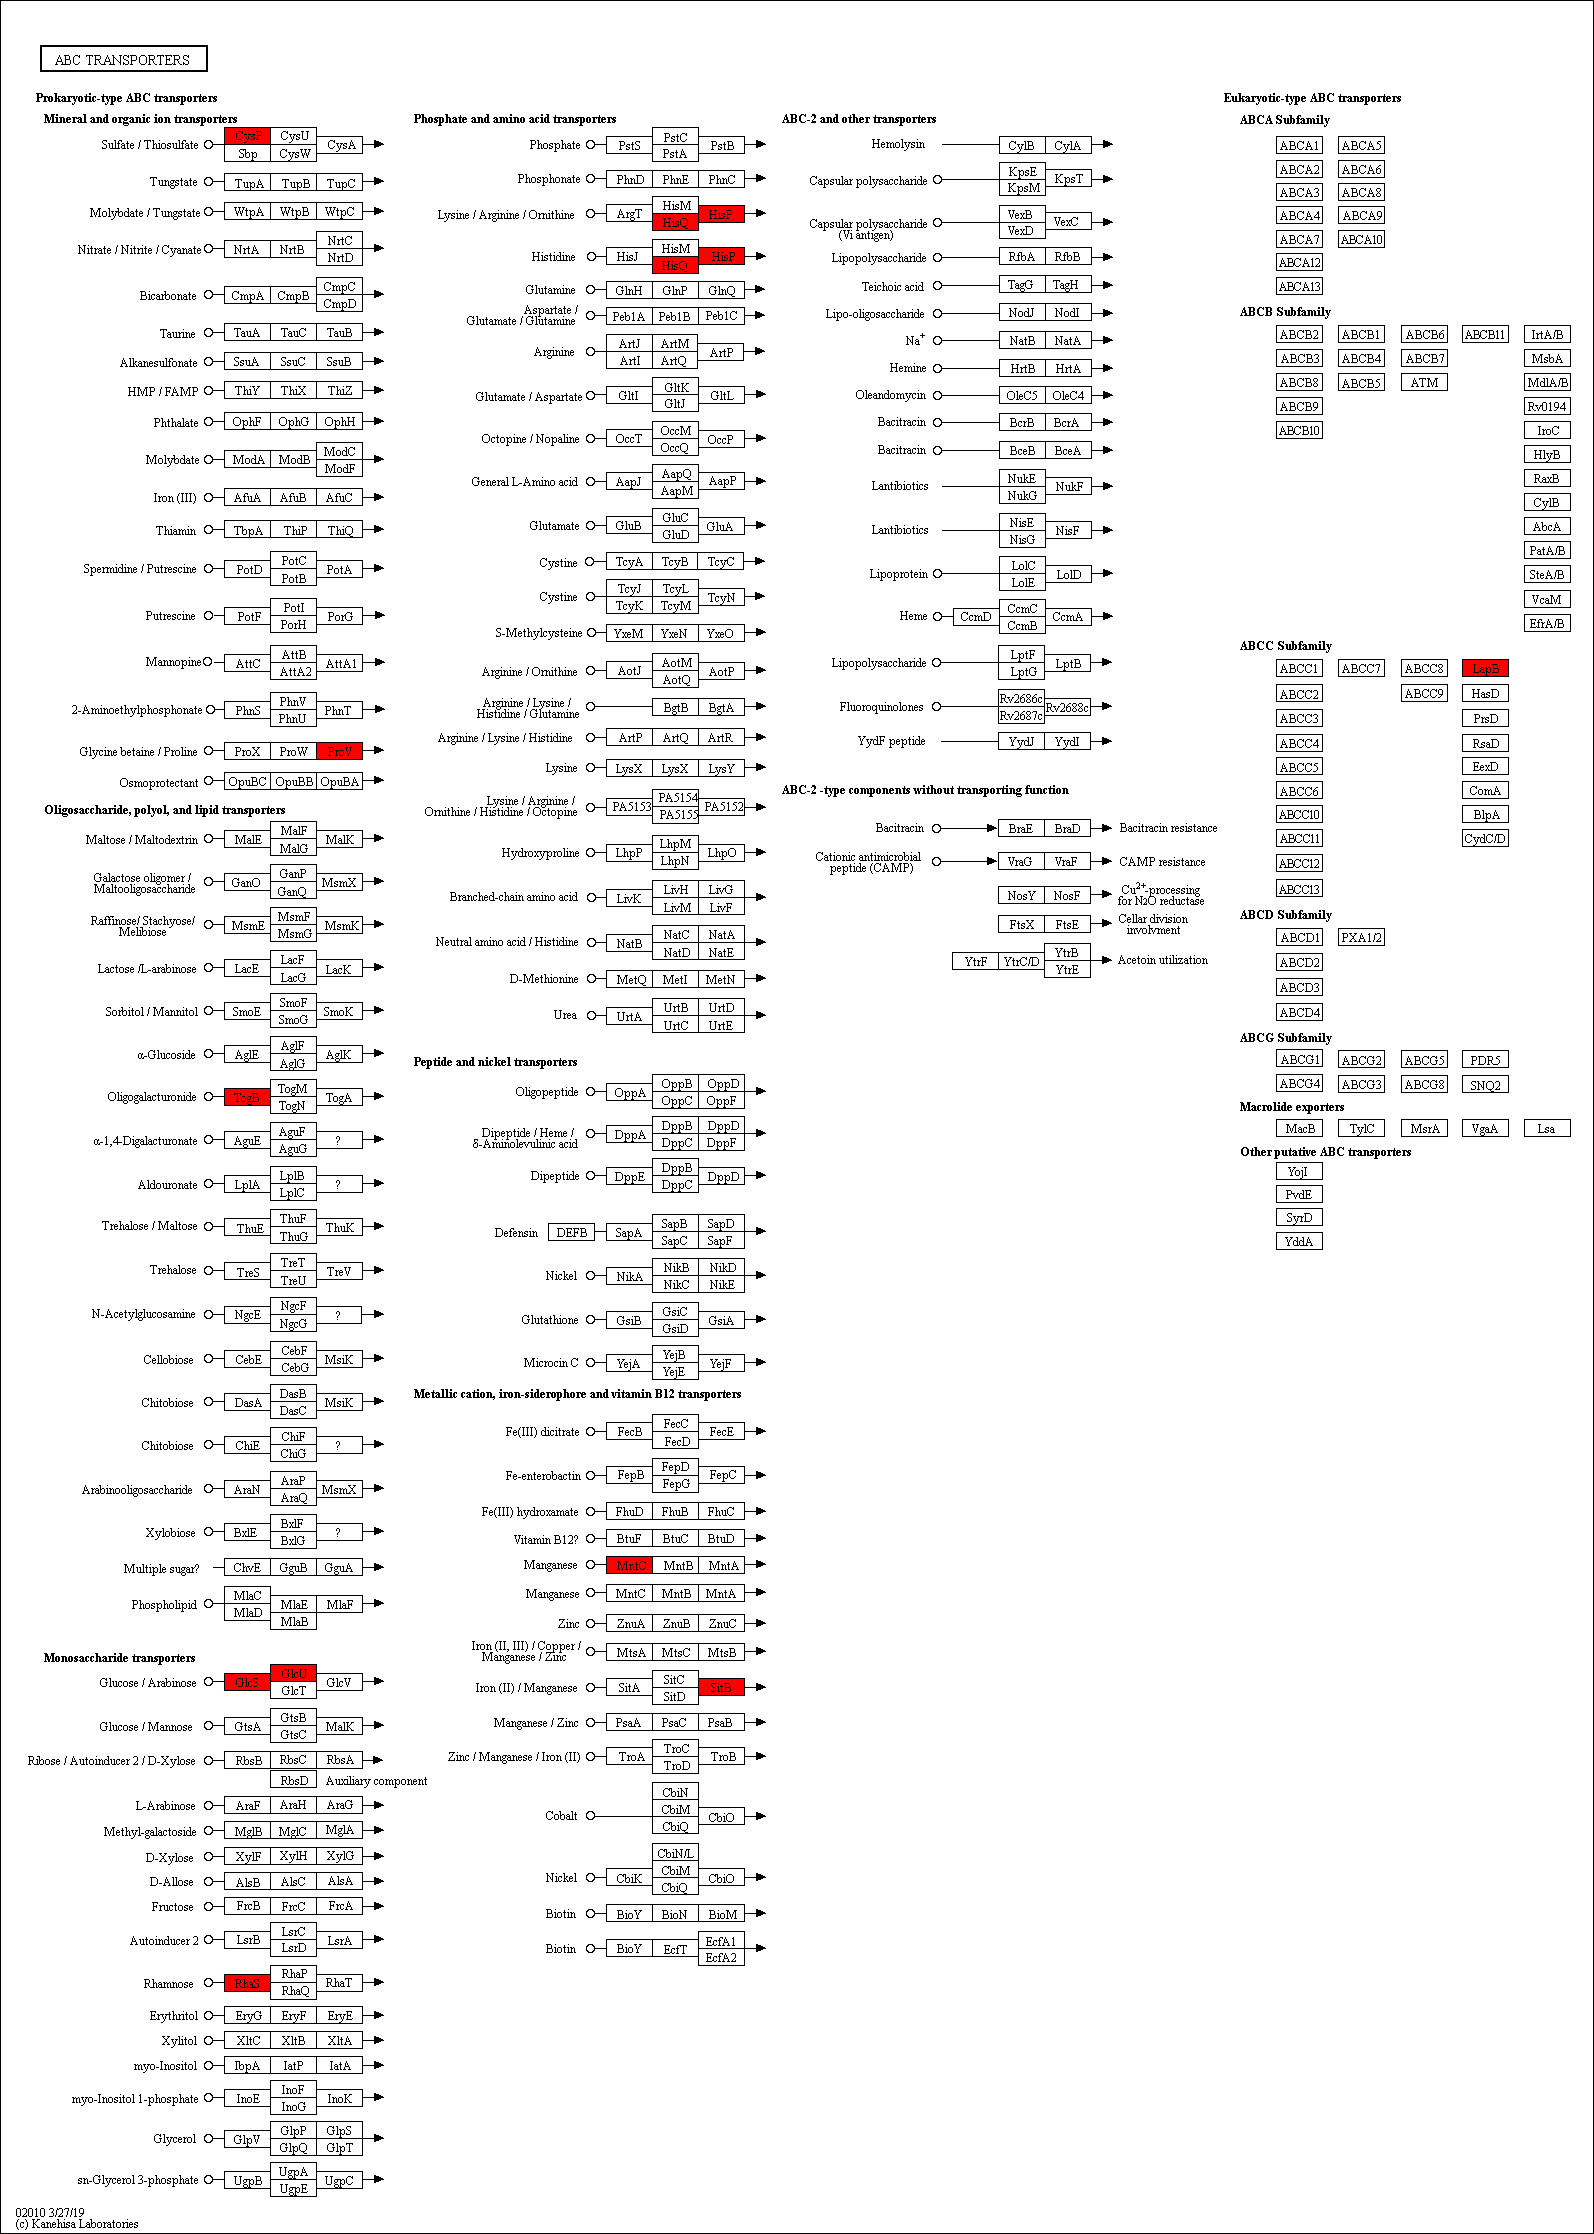
\includegraphics[scale=0.2]{apendices/F-6}
\caption*{\textbf{Anexo F.-} Transportadores ABC presentes en el suelo de la milpa, los genes en rojo presentaron una mayor abundancia respecto a los controles.}
\end{figure}
%\end{landscape}
\chapter{Ruta de pentosas fosfato}
\begin{figure}[!h]
\centering
\centerline{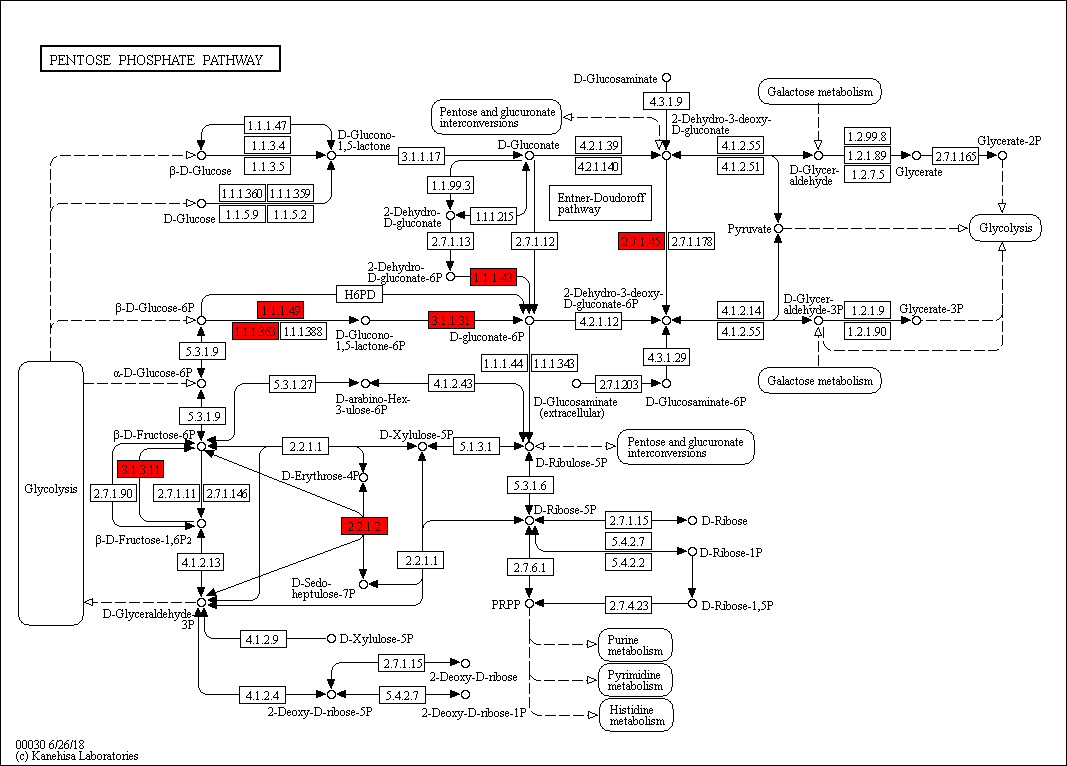
\includegraphics[scale=0.5]{apendices/G-7}}
\caption*{\textbf{Anexo G.-} Ruta metabólica de las pentosas fosfato.}
\end{figure}
\chapter{Ruta de degradación de ácidos grasos}
\begin{figure}[!h]
\centerline{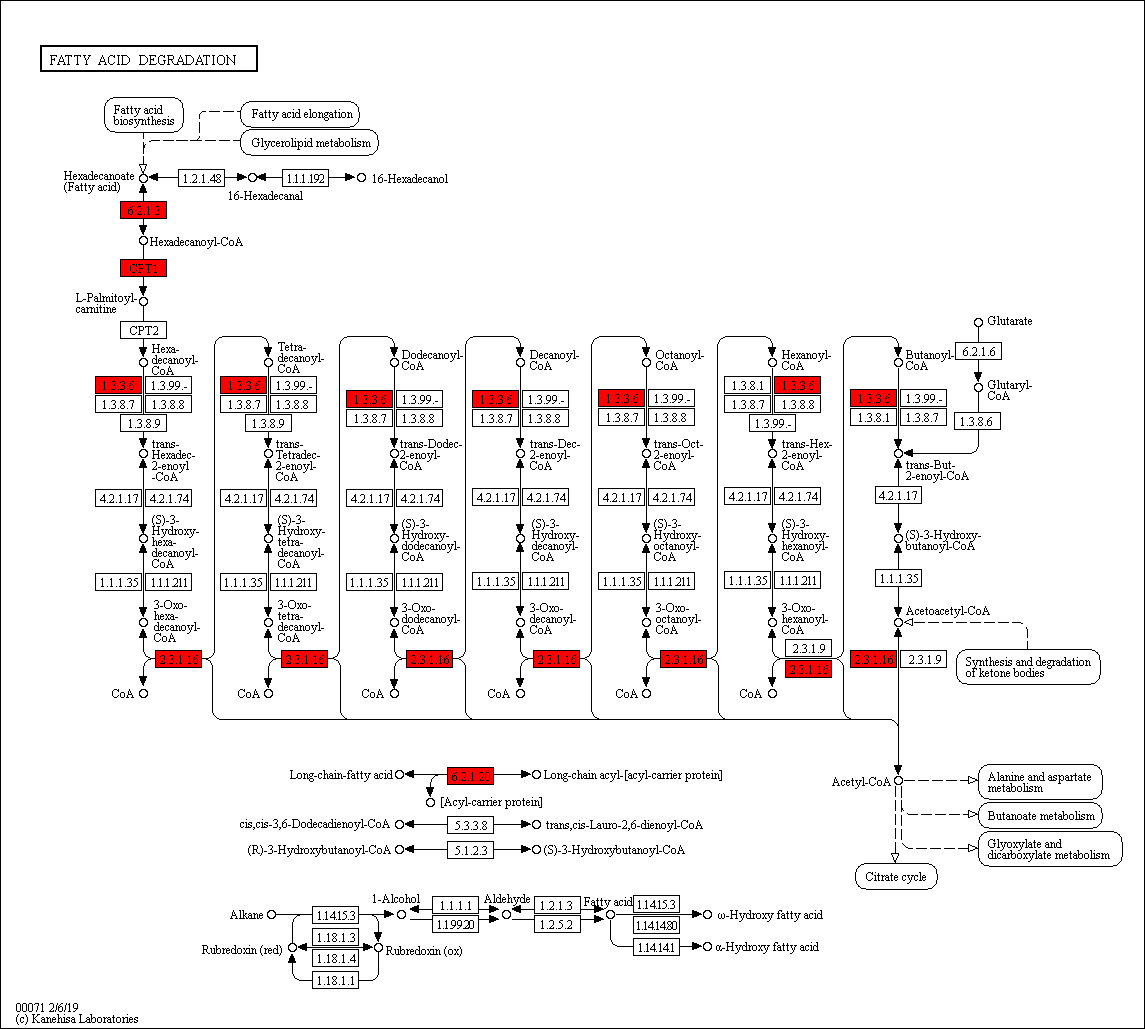
\includegraphics[scale=0.42]{apendices/H-8}}
\caption*{\textbf{Anexo H.-} Ruta metabólica donde se muestran en rojo los genes expresados para la degradación de ácidos grasos.}
\end{figure}
\chapter{Metabolismo del metano}
\begin{figure}[!h]
\centerline{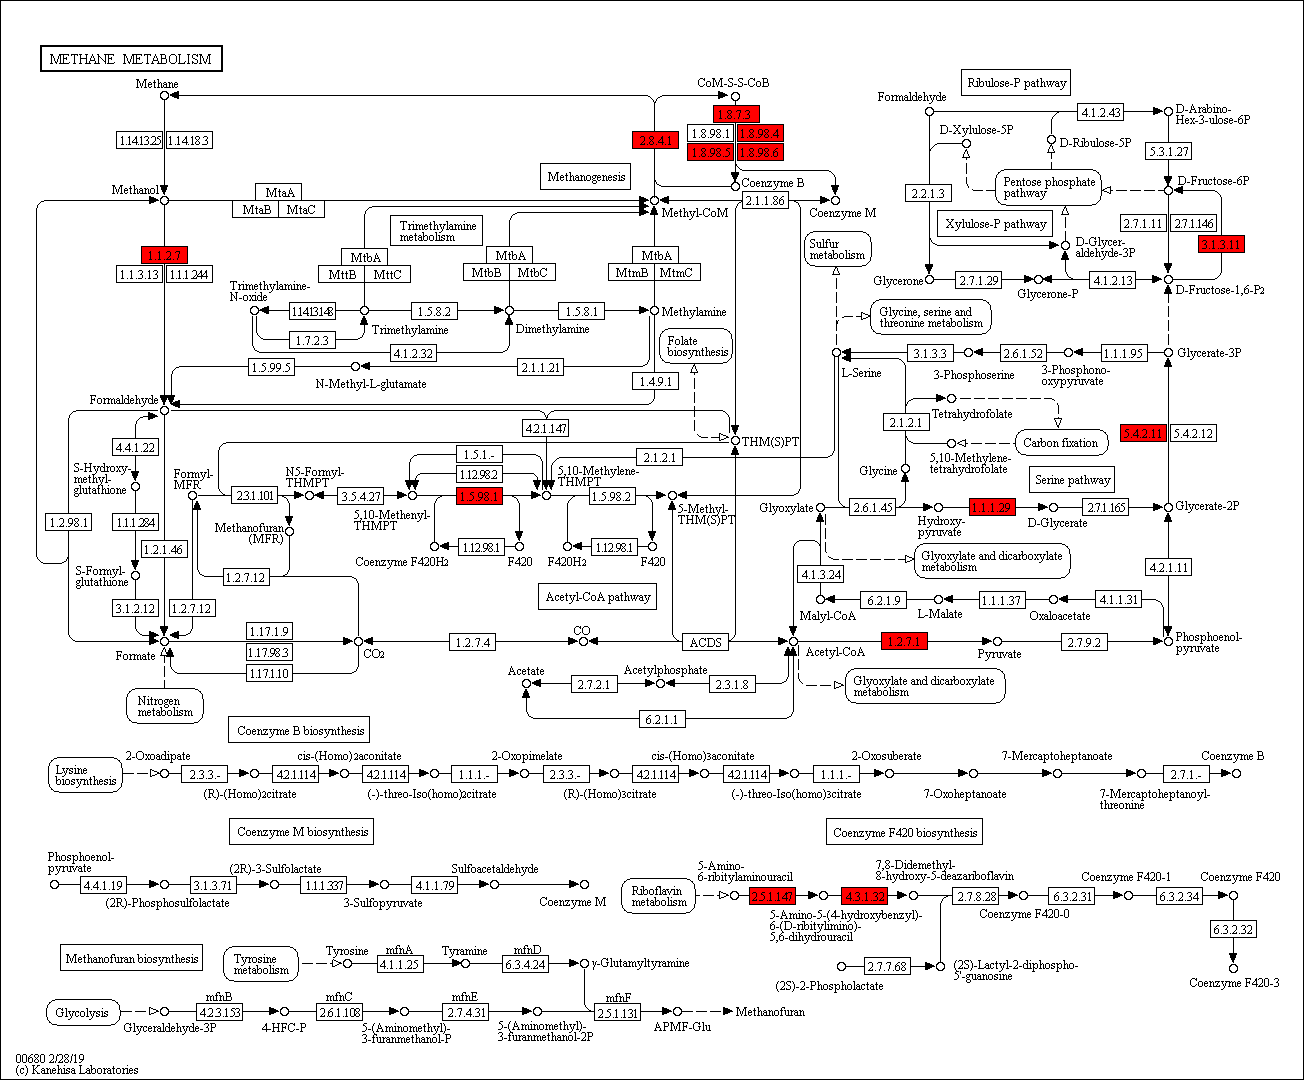
\includegraphics[scale=0.42]{apendices/I-9}}
\caption*{\textbf{Anexo I.-} Ruta metabolica donde se muestra el la degradación del metano donde de rojo se encuentran los genes que lo realizan.}
\end{figure}
\chapter{Ruta del metabolismo del carbono}
\begin{figure}[!h]
\centerline{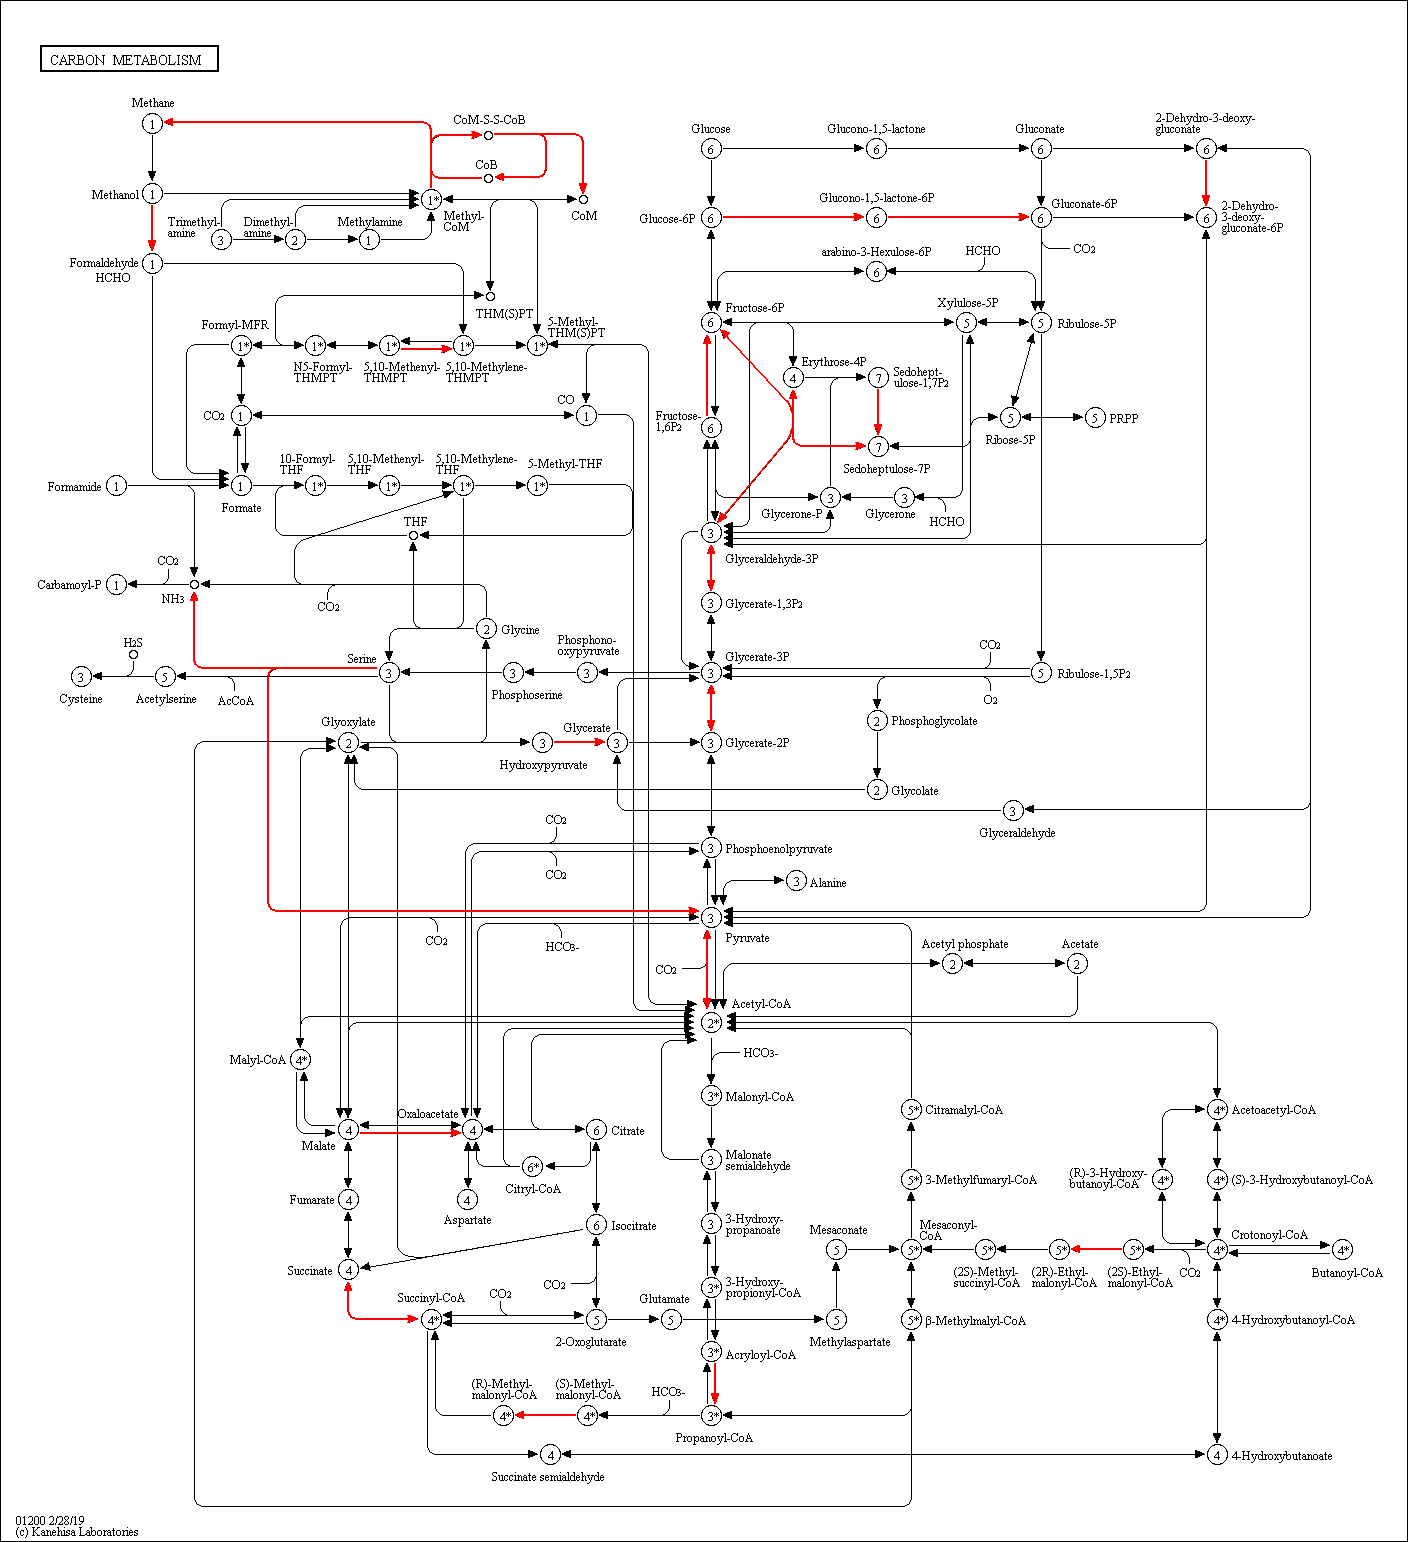
\includegraphics[scale=0.29]{apendices/J-10}}
\caption*{\textbf{Anexo J.-} Ruta donde se muestra el metabolismo del carbono, de rojo se encuentran los genes con mayor abundancia respecto a los controles.}
\end{figure}
\addcontentsline{toc}{chapter}{Bibliografía}
\printbibliography
\end{document}